\documentclass[lettersize,journal]{IEEEtran}
\usepackage{amsmath,amsfonts}
% \usepackage[pagebackref,breaklinks,colorlinks,citecolor=cvprblue]{hyperref}
\usepackage[colorlinks,
            linkcolor=red,
            anchorcolor=blue,
            citecolor=green
            ]{hyperref}
\usepackage{hyperref}
% \usepackage{algorithmic}
\usepackage{algorithm}
\usepackage{array}
\usepackage[caption=false,font=normalsize,labelfont=sf,textfont=sf]{subfig}
\usepackage{textcomp}
\usepackage{stfloats}
\usepackage{url}
\usepackage{verbatim}
\usepackage{graphicx}
\usepackage{cite}
% \usepackage{algorithm2e}
\usepackage{algpseudocode}  
\usepackage[percent]{overpic}
\usepackage{caption}
%\usepackage{xcolor}
% \usepackage[square]{natbib}
\usepackage{enumitem}
\usepackage{tikz}
\usepackage{adjustbox}
\usepackage{cleveref}
\usepackage{multirow}
% \usepackage{abstract}
\hyphenation{op-tical net-works semi-conduc-tor IEEE-Xplore}
% updated with editorial comments 8/9/2021
\renewcommand{\thefootnote}{}

\begin{document}
\title{Part-aware Shape Generation with Latent 3D Diffusion of Neural Voxel Fields}

\author{Yuhang Huang, Shilong Zou, Xinwang Liu,~\IEEEmembership{Senior Member,~IEEE}, Kai Xu$^{*}$\thanks{$*$ Corresponding author (E-mail: kevin.kai.xu@gmail.com).},~\IEEEmembership{Senior Member,~IEEE}
\thanks{The authors are with the School of Computer, National University of Defense Technology, Changsha 410073, China (e-mail: kevin.kai.xu@gmail.com). %X. Xu and X. Chen are with the Hunan University of Technology and Business, Changsha, 410205.
}
% \thanks{This paper was produced by the IEEE Publication Technology Group. They are in Piscataway, NJ.}% <-this % stops a space
% \thanks{Manuscript received April 19, 2021; revised August 16, 2021.}
}

% The paper headers
\markboth{Journal of \LaTeX\ Class Files,~Vol.~14, No.~8, August~2021}%
{Shell \MakeLowercase{\textit{et al.}}: A Sample Article Using IEEEtran.cls for IEEE Journals}

% \IEEEpubid{0000--0000/00\$00.00~\copyright~2021 IEEE}
% Remember, if you use this you must call \IEEEpubidadjcol in the second
% column for its text to clear the IEEEpubid mark.

% \maketitle
% \begin{figure*}[h]
%     \centering
%     % \includegraphics[width=1.\linewidth]{figures/teaser-cvpr.pdf}%\vspace{-10pt}
%     \includegraphics[width=1.\linewidth]{figures/figure1.pdf}%\vspace{-10pt}
%     \caption{High-quality images generated by the proposed DDMs under few-step settings. (a) 10-step unconditioned generation on the CIFAR-10 and CelebA-HQ-256 datasets. (b) 5-step conditioned tasks  %Generated samples on both unconditioned and conditioned tasks. \textbf{(a)}: DDMs can generate high-quality images on CIFAR-10 and CelebA-HQ-256 with only 10 steps. \textbf{(b)}: For conditioned tasks, DDMs only use 5 steps for generating high-quality results 
%     including saliency detection, image inpainting and super-resolution.}%\vspace{-15pt}
%     \label{fig:top}
% \end{figure*}

\maketitle
\begin{abstract}
% This paper presents a novel latent 3D diffusion model for the generation of neural voxel fields, aiming to achieve accurate part-aware structures and high-quality textures. Compared to existing methods, there are two key designs to ensure high-quality and accurate part-aware generation. On one hand, we introduce a latent 3D diffusion process for neural voxel fields, enabling generation at significantly higher resolutions that can accurately capture rich textural and geometric details. On the other hand, a part-aware shape decoder is introduced to integrate the part codes into the neural voxel fields, guiding the accurate part decomposition and producing high-quality rendering results. More importantly, the part-aware learning provides the structural relation guidance for generating texture information of similar regions, facilitating high-quality rendering results. Through extensive experimentation and comparisons with state-of-the-art methods, we evaluate our approach across eight different classes of data. The results demonstrate the superior generative capabilities of our proposed method in part-aware shape generation, outperforming existing state-of-the-art methods.
This paper introduces a novel latent 3D diffusion model for generating neural voxel fields with precise part-aware structures and high-quality textures. In comparison to existing methods, this approach incorporates two key designs to guarantee high-quality and accurate part-aware generation. On one hand, we introduce a latent 3D diffusion process for neural voxel fields, incorporating part-aware information into the diffusion process and allowing generation at significantly higher resolutions to capture rich textural and geometric details accurately. On the other hand, a part-aware shape decoder is introduced to integrate the part codes into the neural voxel fields, guiding accurate part decomposition and producing high-quality rendering results. Importantly, part-aware learning establishes structural relationships to generate texture information for similar regions, thereby facilitating high-quality rendering results. We evaluate our approach across eight different data classes through extensive experimentation and comparisons with state-of-the-art methods. The results demonstrate that our proposed method has superior generative capabilities in part-aware shape generation, outperforming existing state-of-the-art methods. Moreover, we have conducted image- and text-guided shape generation via the conditioned diffusion process, showcasing the advanced potential in multi-modal guided shape generation. %The code will be public at: .
\end{abstract}

\begin{IEEEkeywords}
3D diffusion models, shape generation, part-aware generation.
\end{IEEEkeywords}


\footnote{Q1: We have added the funding in section VI of this manuscript.}
\footnote{Q2: The author affiliations in the first footnote are correct as set.}
\footnote{Q3: Ref.[14]: 1005-1028; Ref.[36]: 8003-8020; Ref.[50]: 3000-3021; Ref.[58]: 50-52.}
\footnote{Q4: The renumbered references are correct as set.}
\footnote{Q5: The renumbered references are correct as set.}

\input{sections/intro}
\input{sections/related_work}
\input{sections/method}
\section{Experiments}
\label{sec:experiments}

We evaluate \methodname{} on two generation paradigms: text-conditioned multi-view generation and action-conditioned multi-view generation. We first describe our implementation details, then present quantitative comparisons against state-of-the-art baselines on three benchmarks.

\subsection{Implementation Details}
\label{sec:impl}

\paragraph{Base Model.}
We build \methodname{} upon the Cosmos-Predict2 diffusion transformer~\cite{nvidia2025cosmos}, a DiT-based world foundation model operating in the latent space of a pretrained video VAE. The Cross-View Attention blocks and Geo-RoPE modules are inserted into the pretrained backbone, while the REPA projection heads are randomly initialized.

\paragraph{Dataset.}
For text-conditioned generation, we train on the AgiBot-World dataset, which provides large-scale multi-view robotic manipulation videos captured from multiple camera viewpoints with paired text descriptions. For action-conditioned generation, we further fine-tune on task-specific data from the AgiBot-Challenge2026 and WorldArena benchmarks.

\paragraph{Training Configuration.}
All experiments are conducted on 200 NVIDIA H200 GPUs. Training proceeds for a total of 30,000 iterations with a batch size proportional to the GPU count. We use the AdamW optimizer with a cosine learning rate schedule. The learning rate warms up linearly over the first 3,000 iterations to peak value $3 \times 10^{-5}$, then decays following a cosine schedule. The full training takes approximately 3 days. The REPA alignment loss weight is set to $\lambda = 0.5$. The 3D foundation model encoders (VGGT~\cite{wang2025vggt} and Depth Anything 3~\cite{lin2025depthanything3}) are kept frozen throughout training.

\subsection{Text-Conditioned Multi-View Generation}
\label{sec:exp-text}

We evaluate text-conditioned generation on the AgiBot-World benchmark, comparing against three state-of-the-art baselines: Genie-Envisioner~\cite{bruce2024genie}, Cosmos-Predict2.5~\cite{nvidia2025cosmos}, and Wan2.2. Results are summarized in \tabref{tab:text-cond}.

\begin{table*}[t]
	\centering
	\caption{Text-conditioned multi-view generation results on the AgiBot-World benchmark. Best results are in \textbf{bold}, second best are \underline{underlined}. $\uparrow$ indicates higher is better, $\downarrow$ indicates lower is better.}
	\label{tab:text-cond}
	\renewcommand{\arraystretch}{1.15}
	\setlength{\tabcolsep}{10pt}
	\begin{tabular}{l c c c c c c c}
		\toprule
		Method & SSIM $\uparrow$ & LPIPS $\downarrow$ & FID $\downarrow$ & FVD $\downarrow$ & Semantic $\uparrow$ & Geometric $\uparrow$ & MEt3R $\downarrow$ \\
		\midrule
		Genie-Envisioner & \underline{0.7445} & 0.3345 & 83.7847 & 207.2025 & \textbf{0.9231} & 0.5327 & \underline{15.75} \\
		Cosmos-Predict2 & 0.5870 & \underline{0.3251} & 58.2837 & 188.6350 & 0.8456 & 0.4824 & 17.47 \\
		Wan2.1 & 0.5715 & 0.3354 & \underline{56.4735} & \underline{174.2186} & 0.8617 & \underline{0.4716} & 16.59 \\
		\textbf{\methodname{} (Ours)} & \textbf{0.7683} & \textbf{0.1844} & \textbf{45.0389} & \textbf{175.7778} & \underline{0.9041} & \textbf{0.4056} & \textbf{14.20} \\
		\bottomrule
	\end{tabular}
\end{table*}

\paragraph{Evaluation Metrics.}
We report seven metrics spanning perceptual quality, distributional fidelity, and 3D geometric consistency:
\begin{itemize}[nosep]
	\item \textbf{SSIM}: Structural similarity measuring pixel-level correspondence.
	\item \textbf{LPIPS}: Learned perceptual similarity in deep feature space (lower is better).
	\item \textbf{FID}: Fr\'echet Inception Distance measuring distributional quality.
	\item \textbf{FVD}: Fr\'echet Video Distance capturing temporal coherence.
	\item \textbf{Semantic}: Semantic consistency score across generated views.
	\item \textbf{Geometric}: Geometric consistency measuring cross-view 3D alignment.
	\item \textbf{MEt3R}: Multi-view 3D reconstruction error (lower is better).
\end{itemize}

\subsection{Action-Conditioned Multi-View Generation}
\label{sec:exp-action}

We further evaluate \methodname{} in the action-conditioned setting, where the model generates future multi-view observations given a sequence of robot actions. This setting directly measures the model's utility as a world simulator for robotic planning and control.

\subsubsection{AgiBot-Challenge2026 Benchmark}

The AgiBot-Challenge2026 benchmark evaluates action-conditioned world models on robotic manipulation tasks with four metrics. Results are reported in \tabref{tab:action-agibot}.

\begin{table}[t]
	\centering
	\caption{Action-conditioned generation results on the AgiBot-Challenge2026 benchmark. Best results are in \textbf{bold}, second best are \underline{underlined}.}
	\label{tab:action-agibot}
	\renewcommand{\arraystretch}{1.15}
	\resizebox{\columnwidth}{!}{%
		\begin{tabular}{lcccc}
			\toprule
			Team & EWMScore $\uparrow$ & PSNR $\uparrow$ & Scene Consistency $\uparrow$ & nDTW $\uparrow$ \\
			\midrule
			NeoVerse-ABot & \textbf{0.829} & \textbf{0.6246} & 0.8974 & \textbf{0.9651} \\
			Loop & 0.8241 & \underline{0.6207} & \underline{0.9024} & 0.9492 \\
			Wild Path & 0.8232 & -- & -- & -- \\
			VIPL-GENUN & 0.8195 & -- & -- & -- \\
			\textbf{\methodname{} (Ours)} & \underline{0.8245} & 0.6161 & \textbf{0.9041} & \underline{0.9531} \\
			\bottomrule
		\end{tabular}%
	}
\end{table}

\paragraph{Evaluation Metrics.}
\begin{itemize}[nosep]
	\item \textbf{EWMScore}: Exponentially Weighted Model Score evaluating overall world model quality.
	\item \textbf{PSNR}: Peak Signal-to-Noise Ratio measuring reconstruction fidelity.
	\item \textbf{Scene Consistency}: Cross-view scene coherence under action conditioning.
	\item \textbf{nDTW}: Normalized Dynamic Time Warping measuring trajectory alignment between generated and ground-truth sequences.
\end{itemize}

\subsubsection{WorldArena Benchmark}

The WorldArena benchmark provides a comprehensive evaluation suite with seven fine-grained metrics that decompose world model quality into distinct dimensions. Results are presented in \tabref{tab:action-worldarena}.

\begin{table*}[t]
	\centering
	\caption{Action-conditioned generation results on the WorldArena benchmark. Best results are in \textbf{bold}, second best are \underline{underlined}.}
	\label{tab:action-worldarena}
	\renewcommand{\arraystretch}{1.15}
	\resizebox{\textwidth}{!}{%
		\begin{tabular}{lccccccc}
			\toprule
			Method & EWMScore $\uparrow$ & Visual Quality $\uparrow$ & Motion Quality $\uparrow$ & Content Consistency $\uparrow$ & Physics Adherence $\uparrow$ & 3D Accuracy $\uparrow$ & Controllability $\uparrow$ \\
			\midrule
			Genie-Envisioner & -- & -- & -- & -- & -- & -- & -- \\
			Cosmos-Predict2.5 & -- & -- & -- & -- & -- & -- & -- \\
			Wan2.2 & -- & -- & -- & -- & -- & -- & -- \\
			\textbf{\methodname{} (Ours)} & \textbf{--} & \textbf{--} & \textbf{--} & \textbf{--} & \textbf{--} & \textbf{--} & \textbf{--} \\
			\bottomrule
		\end{tabular}%
	}
\end{table*}

\paragraph{Evaluation Metrics.}
\begin{itemize}[nosep]
	\item \textbf{EWMScore}: Overall world model quality score.
	\item \textbf{Visual Quality}: Perceptual quality of individual generated frames.
	\item \textbf{Motion Quality}: Smoothness and realism of temporal dynamics.
	\item \textbf{Content Consistency}: Semantic and appearance coherence across frames and views.
	\item \textbf{Physics Adherence}: Physical plausibility of object interactions and dynamics.
	\item \textbf{3D Accuracy}: Geometric correctness of cross-view 3D structure.
	\item \textbf{Controllability}: Fidelity of generated video to the input action commands.
\end{itemize}

\subsection{Ablation Study}
\label{sec:ablation}

To validate our core argument that inter-view communication and 3D geometric priors are both necessary, we conduct ablation experiments systematically removing each component. Results confirm that Cross-View Attention alone or Latent 3D-REPA alone yields limited improvements over the baseline, while their combination produces substantial gains across all metrics.

\section{Conclusion}
\label{sec:conclusion}

We presented \methodname{}, a framework for achieving 3D-consistent multi-view generation in world foundation models for robotic manipulation. Our analysis establishes that multi-view 3D consistency requires two conditions to hold jointly: an inter-view communication mechanism and a 3D geometric prior. Geometry-Aware Cross-View Attention provides the communication channel through which viewpoints exchange information; Latent 3D-REPA supplies the geometric learning signal that steers this exchange toward physically correct 3D representations; and Geometric Rotary Position Embedding encodes camera ray directions and extrinsic poses into the attention mechanism as the common reference frame. We showed that neither condition alone suffices---communication without geometric guidance degenerates into trivial shortcuts, while a geometric prior without an inter-view channel cannot enforce cross-view coherence---and that their combination yields consistent multi-view 3D generation.

Built upon the Cosmos world foundation model~\cite{nvidia2025cosmos}, \methodname{} attains state-of-the-art multi-view 3D consistency on robotic manipulation benchmarks, leading on reconstruction-based, geometric, and scene-consistency metrics across both text- and action-conditioned settings. This improved consistency carries over to downstream embodied tasks: model-based planning benefits from physically plausible imagined trajectories, world action models exhibit stronger action-visual causal alignment, and multi-view policy post-training yields more effective manipulation policies.

Several promising directions remain for future work. First, incorporating \emph{physical interaction modeling}, such as contact dynamics, deformable objects, and fluid simulation, would push 3D consistency beyond geometry into physics-aware world modeling. Second, scaling to \emph{long-horizon planning} scenarios will require maintaining 3D consistency over extended temporal rollouts, potentially through hierarchical or recurrent architectures. Third, by coupling our world model with a World Action Model (WAM), we aim to build a \emph{world-model-driven data closed loop} for embodied intelligence: the world model generates diverse imagined experiences, the WAM learns from these experiences to improve its policy, and the improved policy in turn collects higher-quality real-world data to further refine the world model---enabling continuous self-improvement and autonomous evolution of embodied agents. Fourth, we plan to develop \emph{industrial manufacturing foundation models} built upon our world modeling framework, targeting applications such as dynamic scheduling of production lines and real-time control of manufacturing processes, where accurate physical simulation and multi-view monitoring are critical for intelligent manufacturing.


% \input{appendix/exp_details}
% \begin{thebibliography}{1}
% \nocite{*}
	


\bibliographystyle{IEEEtran} %.bst模板
\bibliography{ref.bib} %.bib文件名字
% \appendices
% \documentclass[lettersize,journal]{IEEEtran}
\usepackage{amsmath,amsfonts}
% \usepackage[pagebackref,breaklinks,colorlinks,citecolor=cvprblue]{hyperref}
\usepackage[colorlinks,
            linkcolor=red,
            anchorcolor=blue,
            citecolor=green
            ]{hyperref}
\usepackage{hyperref}
% \usepackage{algorithmic}
\usepackage{algorithm}
\usepackage{array}
\usepackage[caption=false,font=normalsize,labelfont=sf,textfont=sf]{subfig}
\usepackage{textcomp}
\usepackage{stfloats}
\usepackage{url}
\usepackage{verbatim}
\usepackage{graphicx}
\usepackage{cite}
% \usepackage{algorithm2e}
\usepackage{algpseudocode}  
\usepackage[percent]{overpic}
\usepackage{caption}
%\usepackage{xcolor}
% \usepackage[square]{natbib}
\usepackage{enumitem}
\usepackage{tikz}
\usepackage{adjustbox}
\usepackage{cleveref}
\usepackage{multirow}
% \usepackage{abstract}
\hyphenation{op-tical net-works semi-conduc-tor IEEE-Xplore}
% updated with editorial comments 8/9/2021
\renewcommand{\thefootnote}{}

\begin{document}
\title{Part-aware Shape Generation with Latent 3D Diffusion of Neural Voxel Fields}

\author{Yuhang Huang, Shilong Zou, Xinwang Liu,~\IEEEmembership{Senior Member,~IEEE}, Kai Xu$^{*}$\thanks{$*$ Corresponding author (E-mail: kevin.kai.xu@gmail.com).},~\IEEEmembership{Senior Member,~IEEE}
\thanks{The authors are with the School of Computer, National University of Defense Technology, Changsha 410073, China (e-mail: kevin.kai.xu@gmail.com). %X. Xu and X. Chen are with the Hunan University of Technology and Business, Changsha, 410205.
}
% \thanks{This paper was produced by the IEEE Publication Technology Group. They are in Piscataway, NJ.}% <-this % stops a space
% \thanks{Manuscript received April 19, 2021; revised August 16, 2021.}
}

% The paper headers
\markboth{Journal of \LaTeX\ Class Files,~Vol.~14, No.~8, August~2021}%
{Shell \MakeLowercase{\textit{et al.}}: A Sample Article Using IEEEtran.cls for IEEE Journals}

% \IEEEpubid{0000--0000/00\$00.00~\copyright~2021 IEEE}
% Remember, if you use this you must call \IEEEpubidadjcol in the second
% column for its text to clear the IEEEpubid mark.

% \maketitle
% \begin{figure*}[h]
%     \centering
%     % \includegraphics[width=1.\linewidth]{figures/teaser-cvpr.pdf}%\vspace{-10pt}
%     \includegraphics[width=1.\linewidth]{figures/figure1.pdf}%\vspace{-10pt}
%     \caption{High-quality images generated by the proposed DDMs under few-step settings. (a) 10-step unconditioned generation on the CIFAR-10 and CelebA-HQ-256 datasets. (b) 5-step conditioned tasks  %Generated samples on both unconditioned and conditioned tasks. \textbf{(a)}: DDMs can generate high-quality images on CIFAR-10 and CelebA-HQ-256 with only 10 steps. \textbf{(b)}: For conditioned tasks, DDMs only use 5 steps for generating high-quality results 
%     including saliency detection, image inpainting and super-resolution.}%\vspace{-15pt}
%     \label{fig:top}
% \end{figure*}

\maketitle
\begin{abstract}
% This paper presents a novel latent 3D diffusion model for the generation of neural voxel fields, aiming to achieve accurate part-aware structures and high-quality textures. Compared to existing methods, there are two key designs to ensure high-quality and accurate part-aware generation. On one hand, we introduce a latent 3D diffusion process for neural voxel fields, enabling generation at significantly higher resolutions that can accurately capture rich textural and geometric details. On the other hand, a part-aware shape decoder is introduced to integrate the part codes into the neural voxel fields, guiding the accurate part decomposition and producing high-quality rendering results. More importantly, the part-aware learning provides the structural relation guidance for generating texture information of similar regions, facilitating high-quality rendering results. Through extensive experimentation and comparisons with state-of-the-art methods, we evaluate our approach across eight different classes of data. The results demonstrate the superior generative capabilities of our proposed method in part-aware shape generation, outperforming existing state-of-the-art methods.
This paper introduces a novel latent 3D diffusion model for generating neural voxel fields with precise part-aware structures and high-quality textures. In comparison to existing methods, this approach incorporates two key designs to guarantee high-quality and accurate part-aware generation. On one hand, we introduce a latent 3D diffusion process for neural voxel fields, incorporating part-aware information into the diffusion process and allowing generation at significantly higher resolutions to capture rich textural and geometric details accurately. On the other hand, a part-aware shape decoder is introduced to integrate the part codes into the neural voxel fields, guiding accurate part decomposition and producing high-quality rendering results. Importantly, part-aware learning establishes structural relationships to generate texture information for similar regions, thereby facilitating high-quality rendering results. We evaluate our approach across eight different data classes through extensive experimentation and comparisons with state-of-the-art methods. The results demonstrate that our proposed method has superior generative capabilities in part-aware shape generation, outperforming existing state-of-the-art methods. Moreover, we have conducted image- and text-guided shape generation via the conditioned diffusion process, showcasing the advanced potential in multi-modal guided shape generation. %The code will be public at: .
\end{abstract}

\begin{IEEEkeywords}
3D diffusion models, shape generation, part-aware generation.
\end{IEEEkeywords}


\footnote{Q1: We have added the funding in section VI of this manuscript.}
\footnote{Q2: The author affiliations in the first footnote are correct as set.}
\footnote{Q3: Ref.[14]: 1005-1028; Ref.[36]: 8003-8020; Ref.[50]: 3000-3021; Ref.[58]: 50-52.}
\footnote{Q4: The renumbered references are correct as set.}
\footnote{Q5: The renumbered references are correct as set.}

\input{sections/intro}
\input{sections/related_work}
\input{sections/method}
\section{Experiments}
\label{sec:experiments}

We evaluate \methodname{} on two generation paradigms: text-conditioned multi-view generation and action-conditioned multi-view generation. We first describe our implementation details, then present quantitative comparisons against state-of-the-art baselines on three benchmarks.

\subsection{Implementation Details}
\label{sec:impl}

\paragraph{Base Model.}
We build \methodname{} upon the Cosmos-Predict2 diffusion transformer~\cite{nvidia2025cosmos}, a DiT-based world foundation model operating in the latent space of a pretrained video VAE. The Cross-View Attention blocks and Geo-RoPE modules are inserted into the pretrained backbone, while the REPA projection heads are randomly initialized.

\paragraph{Dataset.}
For text-conditioned generation, we train on the AgiBot-World dataset, which provides large-scale multi-view robotic manipulation videos captured from multiple camera viewpoints with paired text descriptions. For action-conditioned generation, we further fine-tune on task-specific data from the AgiBot-Challenge2026 and WorldArena benchmarks.

\paragraph{Training Configuration.}
All experiments are conducted on 200 NVIDIA H200 GPUs. Training proceeds for a total of 30,000 iterations with a batch size proportional to the GPU count. We use the AdamW optimizer with a cosine learning rate schedule. The learning rate warms up linearly over the first 3,000 iterations to peak value $3 \times 10^{-5}$, then decays following a cosine schedule. The full training takes approximately 3 days. The REPA alignment loss weight is set to $\lambda = 0.5$. The 3D foundation model encoders (VGGT~\cite{wang2025vggt} and Depth Anything 3~\cite{lin2025depthanything3}) are kept frozen throughout training.

\subsection{Text-Conditioned Multi-View Generation}
\label{sec:exp-text}

We evaluate text-conditioned generation on the AgiBot-World benchmark, comparing against three state-of-the-art baselines: Genie-Envisioner~\cite{bruce2024genie}, Cosmos-Predict2.5~\cite{nvidia2025cosmos}, and Wan2.2. Results are summarized in \tabref{tab:text-cond}.

\begin{table*}[t]
	\centering
	\caption{Text-conditioned multi-view generation results on the AgiBot-World benchmark. Best results are in \textbf{bold}, second best are \underline{underlined}. $\uparrow$ indicates higher is better, $\downarrow$ indicates lower is better.}
	\label{tab:text-cond}
	\renewcommand{\arraystretch}{1.15}
	\setlength{\tabcolsep}{10pt}
	\begin{tabular}{l c c c c c c c}
		\toprule
		Method & SSIM $\uparrow$ & LPIPS $\downarrow$ & FID $\downarrow$ & FVD $\downarrow$ & Semantic $\uparrow$ & Geometric $\uparrow$ & MEt3R $\downarrow$ \\
		\midrule
		Genie-Envisioner & \underline{0.7445} & 0.3345 & 83.7847 & 207.2025 & \textbf{0.9231} & 0.5327 & \underline{15.75} \\
		Cosmos-Predict2 & 0.5870 & \underline{0.3251} & 58.2837 & 188.6350 & 0.8456 & 0.4824 & 17.47 \\
		Wan2.1 & 0.5715 & 0.3354 & \underline{56.4735} & \underline{174.2186} & 0.8617 & \underline{0.4716} & 16.59 \\
		\textbf{\methodname{} (Ours)} & \textbf{0.7683} & \textbf{0.1844} & \textbf{45.0389} & \textbf{175.7778} & \underline{0.9041} & \textbf{0.4056} & \textbf{14.20} \\
		\bottomrule
	\end{tabular}
\end{table*}

\paragraph{Evaluation Metrics.}
We report seven metrics spanning perceptual quality, distributional fidelity, and 3D geometric consistency:
\begin{itemize}[nosep]
	\item \textbf{SSIM}: Structural similarity measuring pixel-level correspondence.
	\item \textbf{LPIPS}: Learned perceptual similarity in deep feature space (lower is better).
	\item \textbf{FID}: Fr\'echet Inception Distance measuring distributional quality.
	\item \textbf{FVD}: Fr\'echet Video Distance capturing temporal coherence.
	\item \textbf{Semantic}: Semantic consistency score across generated views.
	\item \textbf{Geometric}: Geometric consistency measuring cross-view 3D alignment.
	\item \textbf{MEt3R}: Multi-view 3D reconstruction error (lower is better).
\end{itemize}

\subsection{Action-Conditioned Multi-View Generation}
\label{sec:exp-action}

We further evaluate \methodname{} in the action-conditioned setting, where the model generates future multi-view observations given a sequence of robot actions. This setting directly measures the model's utility as a world simulator for robotic planning and control.

\subsubsection{AgiBot-Challenge2026 Benchmark}

The AgiBot-Challenge2026 benchmark evaluates action-conditioned world models on robotic manipulation tasks with four metrics. Results are reported in \tabref{tab:action-agibot}.

\begin{table}[t]
	\centering
	\caption{Action-conditioned generation results on the AgiBot-Challenge2026 benchmark. Best results are in \textbf{bold}, second best are \underline{underlined}.}
	\label{tab:action-agibot}
	\renewcommand{\arraystretch}{1.15}
	\resizebox{\columnwidth}{!}{%
		\begin{tabular}{lcccc}
			\toprule
			Team & EWMScore $\uparrow$ & PSNR $\uparrow$ & Scene Consistency $\uparrow$ & nDTW $\uparrow$ \\
			\midrule
			NeoVerse-ABot & \textbf{0.829} & \textbf{0.6246} & 0.8974 & \textbf{0.9651} \\
			Loop & 0.8241 & \underline{0.6207} & \underline{0.9024} & 0.9492 \\
			Wild Path & 0.8232 & -- & -- & -- \\
			VIPL-GENUN & 0.8195 & -- & -- & -- \\
			\textbf{\methodname{} (Ours)} & \underline{0.8245} & 0.6161 & \textbf{0.9041} & \underline{0.9531} \\
			\bottomrule
		\end{tabular}%
	}
\end{table}

\paragraph{Evaluation Metrics.}
\begin{itemize}[nosep]
	\item \textbf{EWMScore}: Exponentially Weighted Model Score evaluating overall world model quality.
	\item \textbf{PSNR}: Peak Signal-to-Noise Ratio measuring reconstruction fidelity.
	\item \textbf{Scene Consistency}: Cross-view scene coherence under action conditioning.
	\item \textbf{nDTW}: Normalized Dynamic Time Warping measuring trajectory alignment between generated and ground-truth sequences.
\end{itemize}

\subsubsection{WorldArena Benchmark}

The WorldArena benchmark provides a comprehensive evaluation suite with seven fine-grained metrics that decompose world model quality into distinct dimensions. Results are presented in \tabref{tab:action-worldarena}.

\begin{table*}[t]
	\centering
	\caption{Action-conditioned generation results on the WorldArena benchmark. Best results are in \textbf{bold}, second best are \underline{underlined}.}
	\label{tab:action-worldarena}
	\renewcommand{\arraystretch}{1.15}
	\resizebox{\textwidth}{!}{%
		\begin{tabular}{lccccccc}
			\toprule
			Method & EWMScore $\uparrow$ & Visual Quality $\uparrow$ & Motion Quality $\uparrow$ & Content Consistency $\uparrow$ & Physics Adherence $\uparrow$ & 3D Accuracy $\uparrow$ & Controllability $\uparrow$ \\
			\midrule
			Genie-Envisioner & -- & -- & -- & -- & -- & -- & -- \\
			Cosmos-Predict2.5 & -- & -- & -- & -- & -- & -- & -- \\
			Wan2.2 & -- & -- & -- & -- & -- & -- & -- \\
			\textbf{\methodname{} (Ours)} & \textbf{--} & \textbf{--} & \textbf{--} & \textbf{--} & \textbf{--} & \textbf{--} & \textbf{--} \\
			\bottomrule
		\end{tabular}%
	}
\end{table*}

\paragraph{Evaluation Metrics.}
\begin{itemize}[nosep]
	\item \textbf{EWMScore}: Overall world model quality score.
	\item \textbf{Visual Quality}: Perceptual quality of individual generated frames.
	\item \textbf{Motion Quality}: Smoothness and realism of temporal dynamics.
	\item \textbf{Content Consistency}: Semantic and appearance coherence across frames and views.
	\item \textbf{Physics Adherence}: Physical plausibility of object interactions and dynamics.
	\item \textbf{3D Accuracy}: Geometric correctness of cross-view 3D structure.
	\item \textbf{Controllability}: Fidelity of generated video to the input action commands.
\end{itemize}

\subsection{Ablation Study}
\label{sec:ablation}

To validate our core argument that inter-view communication and 3D geometric priors are both necessary, we conduct ablation experiments systematically removing each component. Results confirm that Cross-View Attention alone or Latent 3D-REPA alone yields limited improvements over the baseline, while their combination produces substantial gains across all metrics.

\section{Conclusion}
\label{sec:conclusion}

We presented \methodname{}, a framework for achieving 3D-consistent multi-view generation in world foundation models for robotic manipulation. Our analysis establishes that multi-view 3D consistency requires two conditions to hold jointly: an inter-view communication mechanism and a 3D geometric prior. Geometry-Aware Cross-View Attention provides the communication channel through which viewpoints exchange information; Latent 3D-REPA supplies the geometric learning signal that steers this exchange toward physically correct 3D representations; and Geometric Rotary Position Embedding encodes camera ray directions and extrinsic poses into the attention mechanism as the common reference frame. We showed that neither condition alone suffices---communication without geometric guidance degenerates into trivial shortcuts, while a geometric prior without an inter-view channel cannot enforce cross-view coherence---and that their combination yields consistent multi-view 3D generation.

Built upon the Cosmos world foundation model~\cite{nvidia2025cosmos}, \methodname{} attains state-of-the-art multi-view 3D consistency on robotic manipulation benchmarks, leading on reconstruction-based, geometric, and scene-consistency metrics across both text- and action-conditioned settings. This improved consistency carries over to downstream embodied tasks: model-based planning benefits from physically plausible imagined trajectories, world action models exhibit stronger action-visual causal alignment, and multi-view policy post-training yields more effective manipulation policies.

Several promising directions remain for future work. First, incorporating \emph{physical interaction modeling}, such as contact dynamics, deformable objects, and fluid simulation, would push 3D consistency beyond geometry into physics-aware world modeling. Second, scaling to \emph{long-horizon planning} scenarios will require maintaining 3D consistency over extended temporal rollouts, potentially through hierarchical or recurrent architectures. Third, by coupling our world model with a World Action Model (WAM), we aim to build a \emph{world-model-driven data closed loop} for embodied intelligence: the world model generates diverse imagined experiences, the WAM learns from these experiences to improve its policy, and the improved policy in turn collects higher-quality real-world data to further refine the world model---enabling continuous self-improvement and autonomous evolution of embodied agents. Fourth, we plan to develop \emph{industrial manufacturing foundation models} built upon our world modeling framework, targeting applications such as dynamic scheduling of production lines and real-time control of manufacturing processes, where accurate physical simulation and multi-view monitoring are critical for intelligent manufacturing.


% \input{appendix/exp_details}
% \begin{thebibliography}{1}
% \nocite{*}
	


\bibliographystyle{IEEEtran} %.bst模板
\bibliography{ref.bib} %.bib文件名字
% \appendices
% \documentclass[lettersize,journal]{IEEEtran}
\usepackage{amsmath,amsfonts}
% \usepackage[pagebackref,breaklinks,colorlinks,citecolor=cvprblue]{hyperref}
\usepackage[colorlinks,
            linkcolor=red,
            anchorcolor=blue,
            citecolor=green
            ]{hyperref}
\usepackage{hyperref}
% \usepackage{algorithmic}
\usepackage{algorithm}
\usepackage{array}
\usepackage[caption=false,font=normalsize,labelfont=sf,textfont=sf]{subfig}
\usepackage{textcomp}
\usepackage{stfloats}
\usepackage{url}
\usepackage{verbatim}
\usepackage{graphicx}
\usepackage{cite}
% \usepackage{algorithm2e}
\usepackage{algpseudocode}  
\usepackage[percent]{overpic}
\usepackage{caption}
%\usepackage{xcolor}
% \usepackage[square]{natbib}
\usepackage{enumitem}
\usepackage{tikz}
\usepackage{adjustbox}
\usepackage{cleveref}
\usepackage{multirow}
% \usepackage{abstract}
\hyphenation{op-tical net-works semi-conduc-tor IEEE-Xplore}
% updated with editorial comments 8/9/2021
\renewcommand{\thefootnote}{}

\begin{document}
\title{Part-aware Shape Generation with Latent 3D Diffusion of Neural Voxel Fields}

\author{Yuhang Huang, Shilong Zou, Xinwang Liu,~\IEEEmembership{Senior Member,~IEEE}, Kai Xu$^{*}$\thanks{$*$ Corresponding author (E-mail: kevin.kai.xu@gmail.com).},~\IEEEmembership{Senior Member,~IEEE}
\thanks{The authors are with the School of Computer, National University of Defense Technology, Changsha 410073, China (e-mail: kevin.kai.xu@gmail.com). %X. Xu and X. Chen are with the Hunan University of Technology and Business, Changsha, 410205.
}
% \thanks{This paper was produced by the IEEE Publication Technology Group. They are in Piscataway, NJ.}% <-this % stops a space
% \thanks{Manuscript received April 19, 2021; revised August 16, 2021.}
}

% The paper headers
\markboth{Journal of \LaTeX\ Class Files,~Vol.~14, No.~8, August~2021}%
{Shell \MakeLowercase{\textit{et al.}}: A Sample Article Using IEEEtran.cls for IEEE Journals}

% \IEEEpubid{0000--0000/00\$00.00~\copyright~2021 IEEE}
% Remember, if you use this you must call \IEEEpubidadjcol in the second
% column for its text to clear the IEEEpubid mark.

% \maketitle
% \begin{figure*}[h]
%     \centering
%     % \includegraphics[width=1.\linewidth]{figures/teaser-cvpr.pdf}%\vspace{-10pt}
%     \includegraphics[width=1.\linewidth]{figures/figure1.pdf}%\vspace{-10pt}
%     \caption{High-quality images generated by the proposed DDMs under few-step settings. (a) 10-step unconditioned generation on the CIFAR-10 and CelebA-HQ-256 datasets. (b) 5-step conditioned tasks  %Generated samples on both unconditioned and conditioned tasks. \textbf{(a)}: DDMs can generate high-quality images on CIFAR-10 and CelebA-HQ-256 with only 10 steps. \textbf{(b)}: For conditioned tasks, DDMs only use 5 steps for generating high-quality results 
%     including saliency detection, image inpainting and super-resolution.}%\vspace{-15pt}
%     \label{fig:top}
% \end{figure*}

\maketitle
\begin{abstract}
% This paper presents a novel latent 3D diffusion model for the generation of neural voxel fields, aiming to achieve accurate part-aware structures and high-quality textures. Compared to existing methods, there are two key designs to ensure high-quality and accurate part-aware generation. On one hand, we introduce a latent 3D diffusion process for neural voxel fields, enabling generation at significantly higher resolutions that can accurately capture rich textural and geometric details. On the other hand, a part-aware shape decoder is introduced to integrate the part codes into the neural voxel fields, guiding the accurate part decomposition and producing high-quality rendering results. More importantly, the part-aware learning provides the structural relation guidance for generating texture information of similar regions, facilitating high-quality rendering results. Through extensive experimentation and comparisons with state-of-the-art methods, we evaluate our approach across eight different classes of data. The results demonstrate the superior generative capabilities of our proposed method in part-aware shape generation, outperforming existing state-of-the-art methods.
This paper introduces a novel latent 3D diffusion model for generating neural voxel fields with precise part-aware structures and high-quality textures. In comparison to existing methods, this approach incorporates two key designs to guarantee high-quality and accurate part-aware generation. On one hand, we introduce a latent 3D diffusion process for neural voxel fields, incorporating part-aware information into the diffusion process and allowing generation at significantly higher resolutions to capture rich textural and geometric details accurately. On the other hand, a part-aware shape decoder is introduced to integrate the part codes into the neural voxel fields, guiding accurate part decomposition and producing high-quality rendering results. Importantly, part-aware learning establishes structural relationships to generate texture information for similar regions, thereby facilitating high-quality rendering results. We evaluate our approach across eight different data classes through extensive experimentation and comparisons with state-of-the-art methods. The results demonstrate that our proposed method has superior generative capabilities in part-aware shape generation, outperforming existing state-of-the-art methods. Moreover, we have conducted image- and text-guided shape generation via the conditioned diffusion process, showcasing the advanced potential in multi-modal guided shape generation. %The code will be public at: .
\end{abstract}

\begin{IEEEkeywords}
3D diffusion models, shape generation, part-aware generation.
\end{IEEEkeywords}


\footnote{Q1: We have added the funding in section VI of this manuscript.}
\footnote{Q2: The author affiliations in the first footnote are correct as set.}
\footnote{Q3: Ref.[14]: 1005-1028; Ref.[36]: 8003-8020; Ref.[50]: 3000-3021; Ref.[58]: 50-52.}
\footnote{Q4: The renumbered references are correct as set.}
\footnote{Q5: The renumbered references are correct as set.}

\input{sections/intro}
\input{sections/related_work}
\input{sections/method}
\section{Experiments}
\label{sec:experiments}

We evaluate \methodname{} on two generation paradigms: text-conditioned multi-view generation and action-conditioned multi-view generation. We first describe our implementation details, then present quantitative comparisons against state-of-the-art baselines on three benchmarks.

\subsection{Implementation Details}
\label{sec:impl}

\paragraph{Base Model.}
We build \methodname{} upon the Cosmos-Predict2 diffusion transformer~\cite{nvidia2025cosmos}, a DiT-based world foundation model operating in the latent space of a pretrained video VAE. The Cross-View Attention blocks and Geo-RoPE modules are inserted into the pretrained backbone, while the REPA projection heads are randomly initialized.

\paragraph{Dataset.}
For text-conditioned generation, we train on the AgiBot-World dataset, which provides large-scale multi-view robotic manipulation videos captured from multiple camera viewpoints with paired text descriptions. For action-conditioned generation, we further fine-tune on task-specific data from the AgiBot-Challenge2026 and WorldArena benchmarks.

\paragraph{Training Configuration.}
All experiments are conducted on 200 NVIDIA H200 GPUs. Training proceeds for a total of 30,000 iterations with a batch size proportional to the GPU count. We use the AdamW optimizer with a cosine learning rate schedule. The learning rate warms up linearly over the first 3,000 iterations to peak value $3 \times 10^{-5}$, then decays following a cosine schedule. The full training takes approximately 3 days. The REPA alignment loss weight is set to $\lambda = 0.5$. The 3D foundation model encoders (VGGT~\cite{wang2025vggt} and Depth Anything 3~\cite{lin2025depthanything3}) are kept frozen throughout training.

\subsection{Text-Conditioned Multi-View Generation}
\label{sec:exp-text}

We evaluate text-conditioned generation on the AgiBot-World benchmark, comparing against three state-of-the-art baselines: Genie-Envisioner~\cite{bruce2024genie}, Cosmos-Predict2.5~\cite{nvidia2025cosmos}, and Wan2.2. Results are summarized in \tabref{tab:text-cond}.

\begin{table*}[t]
	\centering
	\caption{Text-conditioned multi-view generation results on the AgiBot-World benchmark. Best results are in \textbf{bold}, second best are \underline{underlined}. $\uparrow$ indicates higher is better, $\downarrow$ indicates lower is better.}
	\label{tab:text-cond}
	\renewcommand{\arraystretch}{1.15}
	\setlength{\tabcolsep}{10pt}
	\begin{tabular}{l c c c c c c c}
		\toprule
		Method & SSIM $\uparrow$ & LPIPS $\downarrow$ & FID $\downarrow$ & FVD $\downarrow$ & Semantic $\uparrow$ & Geometric $\uparrow$ & MEt3R $\downarrow$ \\
		\midrule
		Genie-Envisioner & \underline{0.7445} & 0.3345 & 83.7847 & 207.2025 & \textbf{0.9231} & 0.5327 & \underline{15.75} \\
		Cosmos-Predict2 & 0.5870 & \underline{0.3251} & 58.2837 & 188.6350 & 0.8456 & 0.4824 & 17.47 \\
		Wan2.1 & 0.5715 & 0.3354 & \underline{56.4735} & \underline{174.2186} & 0.8617 & \underline{0.4716} & 16.59 \\
		\textbf{\methodname{} (Ours)} & \textbf{0.7683} & \textbf{0.1844} & \textbf{45.0389} & \textbf{175.7778} & \underline{0.9041} & \textbf{0.4056} & \textbf{14.20} \\
		\bottomrule
	\end{tabular}
\end{table*}

\paragraph{Evaluation Metrics.}
We report seven metrics spanning perceptual quality, distributional fidelity, and 3D geometric consistency:
\begin{itemize}[nosep]
	\item \textbf{SSIM}: Structural similarity measuring pixel-level correspondence.
	\item \textbf{LPIPS}: Learned perceptual similarity in deep feature space (lower is better).
	\item \textbf{FID}: Fr\'echet Inception Distance measuring distributional quality.
	\item \textbf{FVD}: Fr\'echet Video Distance capturing temporal coherence.
	\item \textbf{Semantic}: Semantic consistency score across generated views.
	\item \textbf{Geometric}: Geometric consistency measuring cross-view 3D alignment.
	\item \textbf{MEt3R}: Multi-view 3D reconstruction error (lower is better).
\end{itemize}

\subsection{Action-Conditioned Multi-View Generation}
\label{sec:exp-action}

We further evaluate \methodname{} in the action-conditioned setting, where the model generates future multi-view observations given a sequence of robot actions. This setting directly measures the model's utility as a world simulator for robotic planning and control.

\subsubsection{AgiBot-Challenge2026 Benchmark}

The AgiBot-Challenge2026 benchmark evaluates action-conditioned world models on robotic manipulation tasks with four metrics. Results are reported in \tabref{tab:action-agibot}.

\begin{table}[t]
	\centering
	\caption{Action-conditioned generation results on the AgiBot-Challenge2026 benchmark. Best results are in \textbf{bold}, second best are \underline{underlined}.}
	\label{tab:action-agibot}
	\renewcommand{\arraystretch}{1.15}
	\resizebox{\columnwidth}{!}{%
		\begin{tabular}{lcccc}
			\toprule
			Team & EWMScore $\uparrow$ & PSNR $\uparrow$ & Scene Consistency $\uparrow$ & nDTW $\uparrow$ \\
			\midrule
			NeoVerse-ABot & \textbf{0.829} & \textbf{0.6246} & 0.8974 & \textbf{0.9651} \\
			Loop & 0.8241 & \underline{0.6207} & \underline{0.9024} & 0.9492 \\
			Wild Path & 0.8232 & -- & -- & -- \\
			VIPL-GENUN & 0.8195 & -- & -- & -- \\
			\textbf{\methodname{} (Ours)} & \underline{0.8245} & 0.6161 & \textbf{0.9041} & \underline{0.9531} \\
			\bottomrule
		\end{tabular}%
	}
\end{table}

\paragraph{Evaluation Metrics.}
\begin{itemize}[nosep]
	\item \textbf{EWMScore}: Exponentially Weighted Model Score evaluating overall world model quality.
	\item \textbf{PSNR}: Peak Signal-to-Noise Ratio measuring reconstruction fidelity.
	\item \textbf{Scene Consistency}: Cross-view scene coherence under action conditioning.
	\item \textbf{nDTW}: Normalized Dynamic Time Warping measuring trajectory alignment between generated and ground-truth sequences.
\end{itemize}

\subsubsection{WorldArena Benchmark}

The WorldArena benchmark provides a comprehensive evaluation suite with seven fine-grained metrics that decompose world model quality into distinct dimensions. Results are presented in \tabref{tab:action-worldarena}.

\begin{table*}[t]
	\centering
	\caption{Action-conditioned generation results on the WorldArena benchmark. Best results are in \textbf{bold}, second best are \underline{underlined}.}
	\label{tab:action-worldarena}
	\renewcommand{\arraystretch}{1.15}
	\resizebox{\textwidth}{!}{%
		\begin{tabular}{lccccccc}
			\toprule
			Method & EWMScore $\uparrow$ & Visual Quality $\uparrow$ & Motion Quality $\uparrow$ & Content Consistency $\uparrow$ & Physics Adherence $\uparrow$ & 3D Accuracy $\uparrow$ & Controllability $\uparrow$ \\
			\midrule
			Genie-Envisioner & -- & -- & -- & -- & -- & -- & -- \\
			Cosmos-Predict2.5 & -- & -- & -- & -- & -- & -- & -- \\
			Wan2.2 & -- & -- & -- & -- & -- & -- & -- \\
			\textbf{\methodname{} (Ours)} & \textbf{--} & \textbf{--} & \textbf{--} & \textbf{--} & \textbf{--} & \textbf{--} & \textbf{--} \\
			\bottomrule
		\end{tabular}%
	}
\end{table*}

\paragraph{Evaluation Metrics.}
\begin{itemize}[nosep]
	\item \textbf{EWMScore}: Overall world model quality score.
	\item \textbf{Visual Quality}: Perceptual quality of individual generated frames.
	\item \textbf{Motion Quality}: Smoothness and realism of temporal dynamics.
	\item \textbf{Content Consistency}: Semantic and appearance coherence across frames and views.
	\item \textbf{Physics Adherence}: Physical plausibility of object interactions and dynamics.
	\item \textbf{3D Accuracy}: Geometric correctness of cross-view 3D structure.
	\item \textbf{Controllability}: Fidelity of generated video to the input action commands.
\end{itemize}

\subsection{Ablation Study}
\label{sec:ablation}

To validate our core argument that inter-view communication and 3D geometric priors are both necessary, we conduct ablation experiments systematically removing each component. Results confirm that Cross-View Attention alone or Latent 3D-REPA alone yields limited improvements over the baseline, while their combination produces substantial gains across all metrics.

\section{Conclusion}
\label{sec:conclusion}

We presented \methodname{}, a framework for achieving 3D-consistent multi-view generation in world foundation models for robotic manipulation. Our analysis establishes that multi-view 3D consistency requires two conditions to hold jointly: an inter-view communication mechanism and a 3D geometric prior. Geometry-Aware Cross-View Attention provides the communication channel through which viewpoints exchange information; Latent 3D-REPA supplies the geometric learning signal that steers this exchange toward physically correct 3D representations; and Geometric Rotary Position Embedding encodes camera ray directions and extrinsic poses into the attention mechanism as the common reference frame. We showed that neither condition alone suffices---communication without geometric guidance degenerates into trivial shortcuts, while a geometric prior without an inter-view channel cannot enforce cross-view coherence---and that their combination yields consistent multi-view 3D generation.

Built upon the Cosmos world foundation model~\cite{nvidia2025cosmos}, \methodname{} attains state-of-the-art multi-view 3D consistency on robotic manipulation benchmarks, leading on reconstruction-based, geometric, and scene-consistency metrics across both text- and action-conditioned settings. This improved consistency carries over to downstream embodied tasks: model-based planning benefits from physically plausible imagined trajectories, world action models exhibit stronger action-visual causal alignment, and multi-view policy post-training yields more effective manipulation policies.

Several promising directions remain for future work. First, incorporating \emph{physical interaction modeling}, such as contact dynamics, deformable objects, and fluid simulation, would push 3D consistency beyond geometry into physics-aware world modeling. Second, scaling to \emph{long-horizon planning} scenarios will require maintaining 3D consistency over extended temporal rollouts, potentially through hierarchical or recurrent architectures. Third, by coupling our world model with a World Action Model (WAM), we aim to build a \emph{world-model-driven data closed loop} for embodied intelligence: the world model generates diverse imagined experiences, the WAM learns from these experiences to improve its policy, and the improved policy in turn collects higher-quality real-world data to further refine the world model---enabling continuous self-improvement and autonomous evolution of embodied agents. Fourth, we plan to develop \emph{industrial manufacturing foundation models} built upon our world modeling framework, targeting applications such as dynamic scheduling of production lines and real-time control of manufacturing processes, where accurate physical simulation and multi-view monitoring are critical for intelligent manufacturing.


% \input{appendix/exp_details}
% \begin{thebibliography}{1}
% \nocite{*}
	


\bibliographystyle{IEEEtran} %.bst模板
\bibliography{ref.bib} %.bib文件名字
% \appendices
% \documentclass[lettersize,journal]{IEEEtran}
\usepackage{amsmath,amsfonts}
% \usepackage[pagebackref,breaklinks,colorlinks,citecolor=cvprblue]{hyperref}
\usepackage[colorlinks,
            linkcolor=red,
            anchorcolor=blue,
            citecolor=green
            ]{hyperref}
\usepackage{hyperref}
% \usepackage{algorithmic}
\usepackage{algorithm}
\usepackage{array}
\usepackage[caption=false,font=normalsize,labelfont=sf,textfont=sf]{subfig}
\usepackage{textcomp}
\usepackage{stfloats}
\usepackage{url}
\usepackage{verbatim}
\usepackage{graphicx}
\usepackage{cite}
% \usepackage{algorithm2e}
\usepackage{algpseudocode}  
\usepackage[percent]{overpic}
\usepackage{caption}
%\usepackage{xcolor}
% \usepackage[square]{natbib}
\usepackage{enumitem}
\usepackage{tikz}
\usepackage{adjustbox}
\usepackage{cleveref}
\usepackage{multirow}
% \usepackage{abstract}
\hyphenation{op-tical net-works semi-conduc-tor IEEE-Xplore}
% updated with editorial comments 8/9/2021
\renewcommand{\thefootnote}{}

\begin{document}
\title{Part-aware Shape Generation with Latent 3D Diffusion of Neural Voxel Fields}

\author{Yuhang Huang, Shilong Zou, Xinwang Liu,~\IEEEmembership{Senior Member,~IEEE}, Kai Xu$^{*}$\thanks{$*$ Corresponding author (E-mail: kevin.kai.xu@gmail.com).},~\IEEEmembership{Senior Member,~IEEE}
\thanks{The authors are with the School of Computer, National University of Defense Technology, Changsha 410073, China (e-mail: kevin.kai.xu@gmail.com). %X. Xu and X. Chen are with the Hunan University of Technology and Business, Changsha, 410205.
}
% \thanks{This paper was produced by the IEEE Publication Technology Group. They are in Piscataway, NJ.}% <-this % stops a space
% \thanks{Manuscript received April 19, 2021; revised August 16, 2021.}
}

% The paper headers
\markboth{Journal of \LaTeX\ Class Files,~Vol.~14, No.~8, August~2021}%
{Shell \MakeLowercase{\textit{et al.}}: A Sample Article Using IEEEtran.cls for IEEE Journals}

% \IEEEpubid{0000--0000/00\$00.00~\copyright~2021 IEEE}
% Remember, if you use this you must call \IEEEpubidadjcol in the second
% column for its text to clear the IEEEpubid mark.

% \maketitle
% \begin{figure*}[h]
%     \centering
%     % \includegraphics[width=1.\linewidth]{figures/teaser-cvpr.pdf}%\vspace{-10pt}
%     \includegraphics[width=1.\linewidth]{figures/figure1.pdf}%\vspace{-10pt}
%     \caption{High-quality images generated by the proposed DDMs under few-step settings. (a) 10-step unconditioned generation on the CIFAR-10 and CelebA-HQ-256 datasets. (b) 5-step conditioned tasks  %Generated samples on both unconditioned and conditioned tasks. \textbf{(a)}: DDMs can generate high-quality images on CIFAR-10 and CelebA-HQ-256 with only 10 steps. \textbf{(b)}: For conditioned tasks, DDMs only use 5 steps for generating high-quality results 
%     including saliency detection, image inpainting and super-resolution.}%\vspace{-15pt}
%     \label{fig:top}
% \end{figure*}

\maketitle
\begin{abstract}
% This paper presents a novel latent 3D diffusion model for the generation of neural voxel fields, aiming to achieve accurate part-aware structures and high-quality textures. Compared to existing methods, there are two key designs to ensure high-quality and accurate part-aware generation. On one hand, we introduce a latent 3D diffusion process for neural voxel fields, enabling generation at significantly higher resolutions that can accurately capture rich textural and geometric details. On the other hand, a part-aware shape decoder is introduced to integrate the part codes into the neural voxel fields, guiding the accurate part decomposition and producing high-quality rendering results. More importantly, the part-aware learning provides the structural relation guidance for generating texture information of similar regions, facilitating high-quality rendering results. Through extensive experimentation and comparisons with state-of-the-art methods, we evaluate our approach across eight different classes of data. The results demonstrate the superior generative capabilities of our proposed method in part-aware shape generation, outperforming existing state-of-the-art methods.
This paper introduces a novel latent 3D diffusion model for generating neural voxel fields with precise part-aware structures and high-quality textures. In comparison to existing methods, this approach incorporates two key designs to guarantee high-quality and accurate part-aware generation. On one hand, we introduce a latent 3D diffusion process for neural voxel fields, incorporating part-aware information into the diffusion process and allowing generation at significantly higher resolutions to capture rich textural and geometric details accurately. On the other hand, a part-aware shape decoder is introduced to integrate the part codes into the neural voxel fields, guiding accurate part decomposition and producing high-quality rendering results. Importantly, part-aware learning establishes structural relationships to generate texture information for similar regions, thereby facilitating high-quality rendering results. We evaluate our approach across eight different data classes through extensive experimentation and comparisons with state-of-the-art methods. The results demonstrate that our proposed method has superior generative capabilities in part-aware shape generation, outperforming existing state-of-the-art methods. Moreover, we have conducted image- and text-guided shape generation via the conditioned diffusion process, showcasing the advanced potential in multi-modal guided shape generation. %The code will be public at: .
\end{abstract}

\begin{IEEEkeywords}
3D diffusion models, shape generation, part-aware generation.
\end{IEEEkeywords}


\footnote{Q1: We have added the funding in section VI of this manuscript.}
\footnote{Q2: The author affiliations in the first footnote are correct as set.}
\footnote{Q3: Ref.[14]: 1005-1028; Ref.[36]: 8003-8020; Ref.[50]: 3000-3021; Ref.[58]: 50-52.}
\footnote{Q4: The renumbered references are correct as set.}
\footnote{Q5: The renumbered references are correct as set.}

\input{sections/intro}
\input{sections/related_work}
\input{sections/method}
\input{sections/experiment}
\input{sections/conclusion}

% \input{appendix/exp_details}
% \begin{thebibliography}{1}
% \nocite{*}
	


\bibliographystyle{IEEEtran} %.bst模板
\bibliography{ref.bib} %.bib文件名字
% \appendices
% \input{appendix/proof}
% \bibitem{ref1}
% {\it{Mathematics Into Type}}. American Mathematical Society. [Online]. Available: https://www.ams.org/arc/styleguide/mit-2.pdf

% \bibitem{ref2}
% T. W. Chaundy, P. R. Barrett and C. Batey, {\it{The Printing of Mathematics}}. London, U.K., Oxford Univ. Press, 1954.

% \bibitem{ref3}
% F. Mittelbach and M. Goossens, {\it{The \LaTeX Companion}}, 2nd ed. Boston, MA, USA: Pearson, 2004.

% \bibitem{ref4}
% G. Gr\"atzer, {\it{More Math Into LaTeX}}, New York, NY, USA: Springer, 2007.

% \bibitem{ref5}M. Letourneau and J. W. Sharp, {\it{AMS-StyleGuide-online.pdf,}} American Mathematical Society, Providence, RI, USA, [Online]. Available: http://www.ams.org/arc/styleguide/index.html

% \bibitem{ref6}
% H. Sira-Ramirez, ``On the sliding mode control of nonlinear systems,'' \textit{Syst. Control Lett.}, vol. 19, pp. 303--312, 1992.

% \bibitem{ref7}
% A. Levant, ``Exact differentiation of signals with unbounded higher derivatives,''  in \textit{Proc. 45th IEEE Conf. Decis.
% Control}, San Diego, CA, USA, 2006, pp. 5585--5590. DOI: 10.1109/CDC.2006.377165.

% \bibitem{ref8}
% M. Fliess, C. Join, and H. Sira-Ramirez, ``Non-linear estimation is easy,'' \textit{Int. J. Model., Ident. Control}, vol. 4, no. 1, pp. 12--27, 2008.

% \bibitem{ref9}
% R. Ortega, A. Astolfi, G. Bastin, and H. Rodriguez, ``Stabilization of food-chain systems using a port-controlled Hamiltonian description,'' in \textit{Proc. Amer. Control Conf.}, Chicago, IL, USA,
% 2000, pp. 2245--2249.

% \end{thebibliography}


\newpage

 
\vspace{11pt}

% \bf{If you include a photo:}\vspace{-33pt}
\begin{IEEEbiography}[{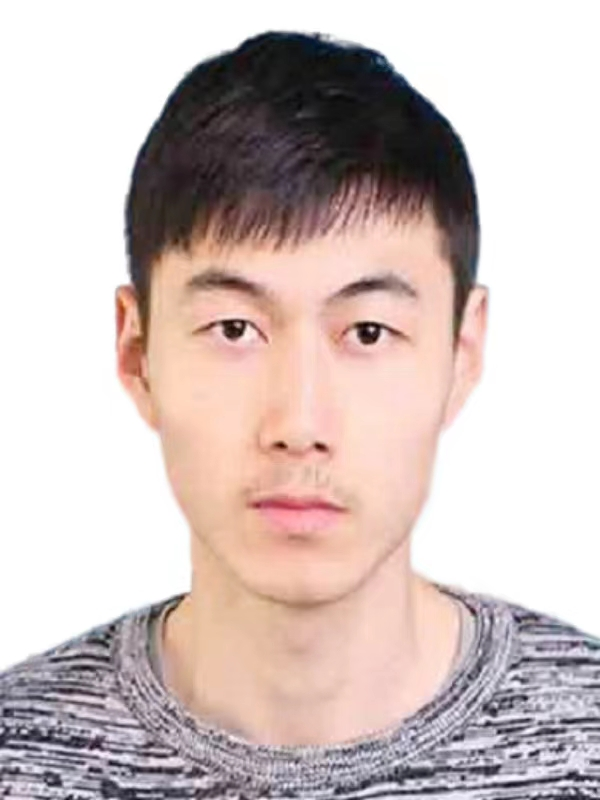
\includegraphics[width=1in,height=1.25in,clip,keepaspectratio]{figures/hyx.jpg}}]{Yuhang Huang}
received the bachelor’s degree from the University of Shanghai for Science and Technology, Shanghai, China, in 2019, and the master’s degree from Shanghai University, Shanghai, China, in 2022. He is currently pursuing the Ph.D. degree at the National University of Defense Technology, Changsha, China.

His research interests include computer vision, graphics, and generative models.
\end{IEEEbiography}


\vspace{11pt}
\begin{IEEEbiography}[{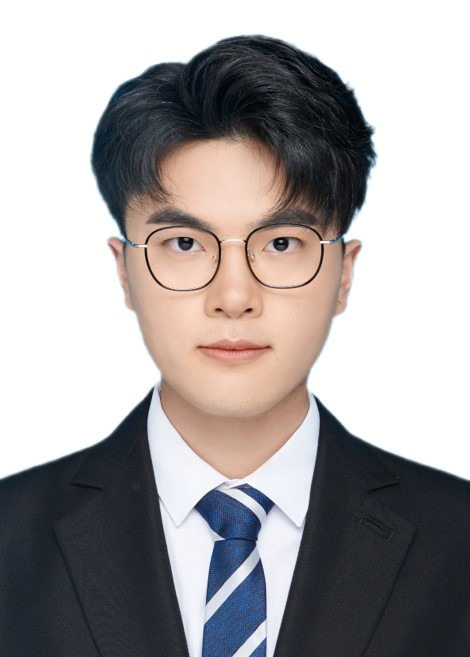
\includegraphics[width=1in,height=1.25in,clip,keepaspectratio]{figures/zsl.jpg}}]{Shilong Zou} received the bachelor's degree from the University of Dalian Maritime University, Dalian, 2023. He is currently pursuing the master's degree at the National University of Defense Technology, Changsha, China. 

His research interests include computer vision and generative models.
\end{IEEEbiography}
% \bf{If you will not include a photo:}\vspace{-33pt}
% \begin{IEEEbiographynophoto}{John Doe}
% Use $\backslash${\tt{begin\{IEEEbiographynophoto\}}} and the author name as the argument followed by the biography text.
% \end{IEEEbiographynophoto}
% \begin{IEEEbiography}[{\includegraphics[width=1in,height=1.25in,clip,keepaspectratio]{figures/qinzheng.jpg}}]{Zheng Qin} 
% received the PhD degree in computer science and technology from National University of Defense Technology (NUDT), China. He is currently an assistant professor with the Defense Innovation Institute, Academy of Military Sciences, China. His current research interests include 3D computer vision, 3D feature learning, shape modeling, and scene understanding.
% \end{IEEEbiography} 

% \vspace{11pt}
% \begin{IEEEbiography}[{\includegraphics[width=1in,height=1.25in,clip,keepaspectratio]{figures/xuesongxu.png}}]{Xuesong Xu} received his M.S and
% Ph.D. degree in Control Science and
% Engineering from Hunan University in
% 2004 and 2009 respectively. From 2012 to
% 2015, he works as a post-doctoral at
% National University of defense and
% technology. From 2016-2017, he also
% works as a visiting researcher in Volen
% National Center for Complex Systems,
% Brandeis University, USA. Currently, He is a professor of
% Hunan University of Technology and Business, working at
% Base of International Science and Technology Innovation and
% Cooperation on Big Data Technology and Management. His
% research interests are in the areas of complex system
% optimization, Blockchain and Machine learning. He has
% published more than 30 papers at various conferences and
% journals, including FGCS, Energy Reports, and Sensors. Prof.
% Xu is a member of the IEEE Computational Intelligence.
% \end{IEEEbiography}

% \vspace{11pt}
% \begin{IEEEbiography}[{\includegraphics[width=1in,height=1.25in,clip,keepaspectratio]{figures/zhuchengyang.png}}]{Chengyang Zhu} is an Associate Professor at the School of Computer, National University of Defense
% Technology. The current directions of interest include data-driven shape analysis and modeling, 3D vision and, robot perception \& navigation, etc.
% \end{IEEEbiography}

\vspace{11pt}
\begin{IEEEbiography}[{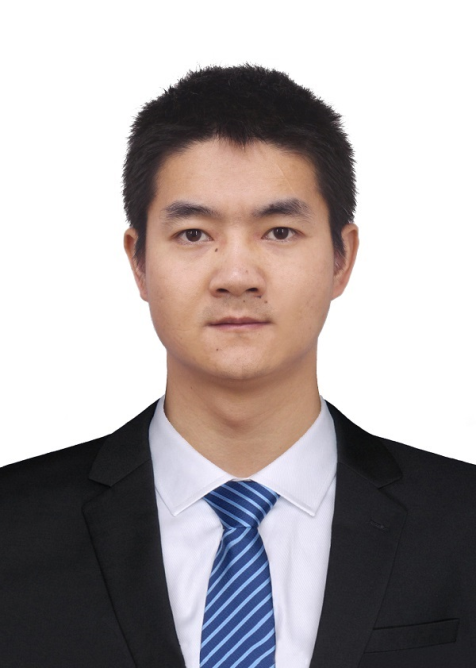
\includegraphics[width=1in,height=1.25in,clip,keepaspectratio]{figures/lxw.png}}]{Xinwang Liu}
received his PhD degree from National University of Defense Technology (NUDT), China. He is now Professor of School of Computer, NUDT. His current research interests include kernel learning and unsupervised feature learning. Dr. Liu has published 60+ peer-reviewed papers, including
those in highly regarded journals and conferences such as IEEE T-PAMI, IEEE T-KDE, IEEE T-IP, IEEE T-NNLS, IEEE T-MM, IEEE T-IFS, ICML, NeurIPS, ICCV, CVPR, AAAI, IJCAI, etc. He serves as the associated editor of Information Fusion Journal. More information can be found at \href{https://xinwangliu.github.io/}{https://xinwangliu.github.io/}.
\end{IEEEbiography}

% \begin{IEEEbiography}
% [{\includegraphics[width=1in,height=1.25in,clip,keepaspectratio]{figures/xiaohongchen.png}}]{Xiaohong Chen} 
% is an Academician of the Chinese Academy of Engineering and is a Distinguished Expert of Management Science and Engineering, Engineering Management, and Data Intelligence. Additionally, she is the Convener of the Management Science and Engineering Discipline Assessment Group under the Degree Committee of the State Council, the Director of the National Basic Science Center, and the Director of the Xiangjiang Laboratory, Changsha, China. Her leadership roles extend to the Innovation Group of the National Natural Science Foundation, the Cheung Kong Scholars Innovation Team under the Ministry of Education, and as a Leading Talent of Philosophy and Social Sciences in the Ten Thousand Talents Plan of the Organization Department of the Central Committee of the People’s Republic of China. She has published over 400 papers in prestigious academic journals, with more than 60 papers featured in the top 1\% of ESI highly cited papers, and holds an H-Index of 87. Her research focuses on decision theory and decision support systems, data intelligence, and the advancement of a smart society.
% \end{IEEEbiography}

\vspace{11pt}
\begin{IEEEbiography}[{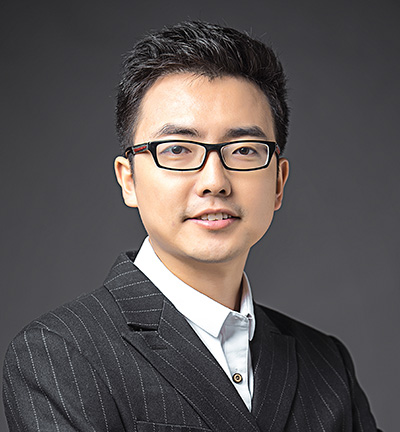
\includegraphics[width=1in,height=1.25in,clip,keepaspectratio]{figures/kevinxu.jpg}}]{Kai Xu} (Senior Member, IEEE) received the Ph.D. degree in computer science from the National University of Defense Technology (NUDT), Changsha,
China, in 2011. From 2008 to 2010, he worked as a Visiting Ph.D. degree with the GrUVi Laboratory, Simon Fraser University, Burnaby, BC, Canada. He is currently a Professor with the School of Computer Science, NUDT. He is also an Adjunct Professor with Simon Fraser University. His current research interests include data-driven shape analysis and modeling, and 3-D vision and robot perception and navigation.
\end{IEEEbiography}




\vfill

\end{document}



% \bibitem{ref1}
% {\it{Mathematics Into Type}}. American Mathematical Society. [Online]. Available: https://www.ams.org/arc/styleguide/mit-2.pdf

% \bibitem{ref2}
% T. W. Chaundy, P. R. Barrett and C. Batey, {\it{The Printing of Mathematics}}. London, U.K., Oxford Univ. Press, 1954.

% \bibitem{ref3}
% F. Mittelbach and M. Goossens, {\it{The \LaTeX Companion}}, 2nd ed. Boston, MA, USA: Pearson, 2004.

% \bibitem{ref4}
% G. Gr\"atzer, {\it{More Math Into LaTeX}}, New York, NY, USA: Springer, 2007.

% \bibitem{ref5}M. Letourneau and J. W. Sharp, {\it{AMS-StyleGuide-online.pdf,}} American Mathematical Society, Providence, RI, USA, [Online]. Available: http://www.ams.org/arc/styleguide/index.html

% \bibitem{ref6}
% H. Sira-Ramirez, ``On the sliding mode control of nonlinear systems,'' \textit{Syst. Control Lett.}, vol. 19, pp. 303--312, 1992.

% \bibitem{ref7}
% A. Levant, ``Exact differentiation of signals with unbounded higher derivatives,''  in \textit{Proc. 45th IEEE Conf. Decis.
% Control}, San Diego, CA, USA, 2006, pp. 5585--5590. DOI: 10.1109/CDC.2006.377165.

% \bibitem{ref8}
% M. Fliess, C. Join, and H. Sira-Ramirez, ``Non-linear estimation is easy,'' \textit{Int. J. Model., Ident. Control}, vol. 4, no. 1, pp. 12--27, 2008.

% \bibitem{ref9}
% R. Ortega, A. Astolfi, G. Bastin, and H. Rodriguez, ``Stabilization of food-chain systems using a port-controlled Hamiltonian description,'' in \textit{Proc. Amer. Control Conf.}, Chicago, IL, USA,
% 2000, pp. 2245--2249.

% \end{thebibliography}


\newpage

 
\vspace{11pt}

% \bf{If you include a photo:}\vspace{-33pt}
\begin{IEEEbiography}[{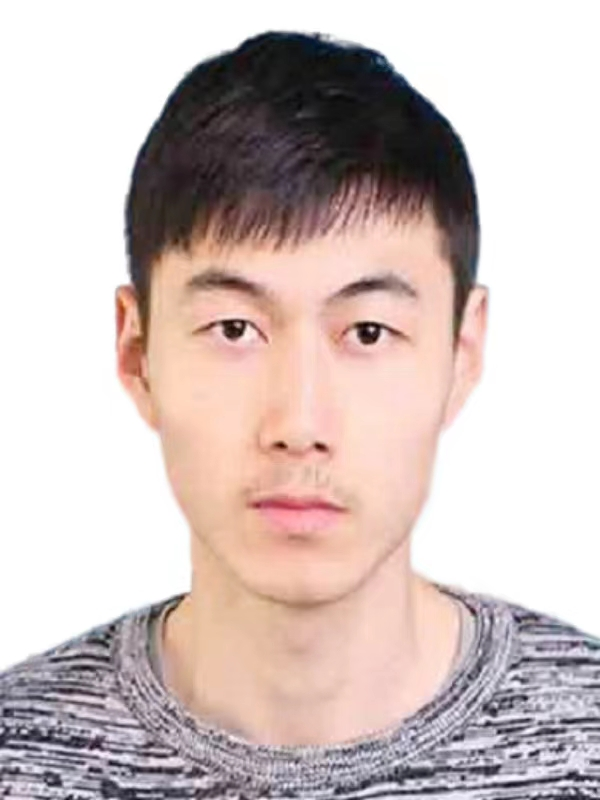
\includegraphics[width=1in,height=1.25in,clip,keepaspectratio]{figures/hyx.jpg}}]{Yuhang Huang}
received the bachelor’s degree from the University of Shanghai for Science and Technology, Shanghai, China, in 2019, and the master’s degree from Shanghai University, Shanghai, China, in 2022. He is currently pursuing the Ph.D. degree at the National University of Defense Technology, Changsha, China.

His research interests include computer vision, graphics, and generative models.
\end{IEEEbiography}


\vspace{11pt}
\begin{IEEEbiography}[{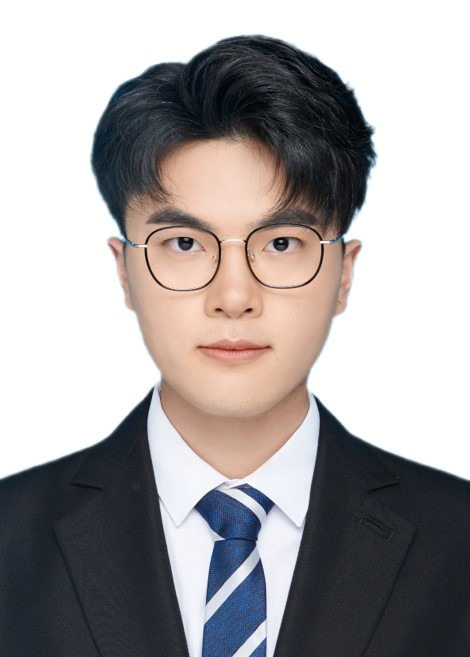
\includegraphics[width=1in,height=1.25in,clip,keepaspectratio]{figures/zsl.jpg}}]{Shilong Zou} received the bachelor's degree from the University of Dalian Maritime University, Dalian, 2023. He is currently pursuing the master's degree at the National University of Defense Technology, Changsha, China. 

His research interests include computer vision and generative models.
\end{IEEEbiography}
% \bf{If you will not include a photo:}\vspace{-33pt}
% \begin{IEEEbiographynophoto}{John Doe}
% Use $\backslash${\tt{begin\{IEEEbiographynophoto\}}} and the author name as the argument followed by the biography text.
% \end{IEEEbiographynophoto}
% \begin{IEEEbiography}[{\includegraphics[width=1in,height=1.25in,clip,keepaspectratio]{figures/qinzheng.jpg}}]{Zheng Qin} 
% received the PhD degree in computer science and technology from National University of Defense Technology (NUDT), China. He is currently an assistant professor with the Defense Innovation Institute, Academy of Military Sciences, China. His current research interests include 3D computer vision, 3D feature learning, shape modeling, and scene understanding.
% \end{IEEEbiography} 

% \vspace{11pt}
% \begin{IEEEbiography}[{\includegraphics[width=1in,height=1.25in,clip,keepaspectratio]{figures/xuesongxu.png}}]{Xuesong Xu} received his M.S and
% Ph.D. degree in Control Science and
% Engineering from Hunan University in
% 2004 and 2009 respectively. From 2012 to
% 2015, he works as a post-doctoral at
% National University of defense and
% technology. From 2016-2017, he also
% works as a visiting researcher in Volen
% National Center for Complex Systems,
% Brandeis University, USA. Currently, He is a professor of
% Hunan University of Technology and Business, working at
% Base of International Science and Technology Innovation and
% Cooperation on Big Data Technology and Management. His
% research interests are in the areas of complex system
% optimization, Blockchain and Machine learning. He has
% published more than 30 papers at various conferences and
% journals, including FGCS, Energy Reports, and Sensors. Prof.
% Xu is a member of the IEEE Computational Intelligence.
% \end{IEEEbiography}

% \vspace{11pt}
% \begin{IEEEbiography}[{\includegraphics[width=1in,height=1.25in,clip,keepaspectratio]{figures/zhuchengyang.png}}]{Chengyang Zhu} is an Associate Professor at the School of Computer, National University of Defense
% Technology. The current directions of interest include data-driven shape analysis and modeling, 3D vision and, robot perception \& navigation, etc.
% \end{IEEEbiography}

\vspace{11pt}
\begin{IEEEbiography}[{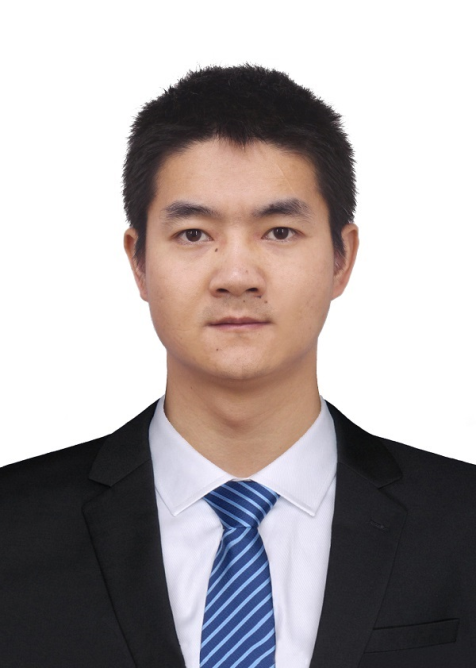
\includegraphics[width=1in,height=1.25in,clip,keepaspectratio]{figures/lxw.png}}]{Xinwang Liu}
received his PhD degree from National University of Defense Technology (NUDT), China. He is now Professor of School of Computer, NUDT. His current research interests include kernel learning and unsupervised feature learning. Dr. Liu has published 60+ peer-reviewed papers, including
those in highly regarded journals and conferences such as IEEE T-PAMI, IEEE T-KDE, IEEE T-IP, IEEE T-NNLS, IEEE T-MM, IEEE T-IFS, ICML, NeurIPS, ICCV, CVPR, AAAI, IJCAI, etc. He serves as the associated editor of Information Fusion Journal. More information can be found at \href{https://xinwangliu.github.io/}{https://xinwangliu.github.io/}.
\end{IEEEbiography}

% \begin{IEEEbiography}
% [{\includegraphics[width=1in,height=1.25in,clip,keepaspectratio]{figures/xiaohongchen.png}}]{Xiaohong Chen} 
% is an Academician of the Chinese Academy of Engineering and is a Distinguished Expert of Management Science and Engineering, Engineering Management, and Data Intelligence. Additionally, she is the Convener of the Management Science and Engineering Discipline Assessment Group under the Degree Committee of the State Council, the Director of the National Basic Science Center, and the Director of the Xiangjiang Laboratory, Changsha, China. Her leadership roles extend to the Innovation Group of the National Natural Science Foundation, the Cheung Kong Scholars Innovation Team under the Ministry of Education, and as a Leading Talent of Philosophy and Social Sciences in the Ten Thousand Talents Plan of the Organization Department of the Central Committee of the People’s Republic of China. She has published over 400 papers in prestigious academic journals, with more than 60 papers featured in the top 1\% of ESI highly cited papers, and holds an H-Index of 87. Her research focuses on decision theory and decision support systems, data intelligence, and the advancement of a smart society.
% \end{IEEEbiography}

\vspace{11pt}
\begin{IEEEbiography}[{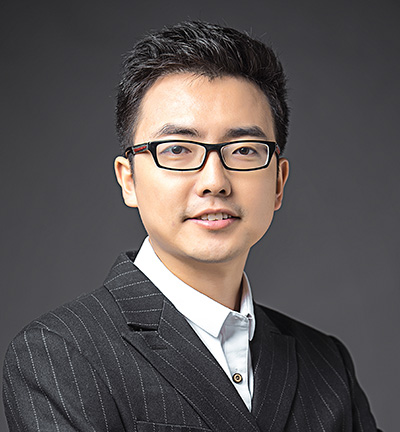
\includegraphics[width=1in,height=1.25in,clip,keepaspectratio]{figures/kevinxu.jpg}}]{Kai Xu} (Senior Member, IEEE) received the Ph.D. degree in computer science from the National University of Defense Technology (NUDT), Changsha,
China, in 2011. From 2008 to 2010, he worked as a Visiting Ph.D. degree with the GrUVi Laboratory, Simon Fraser University, Burnaby, BC, Canada. He is currently a Professor with the School of Computer Science, NUDT. He is also an Adjunct Professor with Simon Fraser University. His current research interests include data-driven shape analysis and modeling, and 3-D vision and robot perception and navigation.
\end{IEEEbiography}




\vfill

\end{document}



% \bibitem{ref1}
% {\it{Mathematics Into Type}}. American Mathematical Society. [Online]. Available: https://www.ams.org/arc/styleguide/mit-2.pdf

% \bibitem{ref2}
% T. W. Chaundy, P. R. Barrett and C. Batey, {\it{The Printing of Mathematics}}. London, U.K., Oxford Univ. Press, 1954.

% \bibitem{ref3}
% F. Mittelbach and M. Goossens, {\it{The \LaTeX Companion}}, 2nd ed. Boston, MA, USA: Pearson, 2004.

% \bibitem{ref4}
% G. Gr\"atzer, {\it{More Math Into LaTeX}}, New York, NY, USA: Springer, 2007.

% \bibitem{ref5}M. Letourneau and J. W. Sharp, {\it{AMS-StyleGuide-online.pdf,}} American Mathematical Society, Providence, RI, USA, [Online]. Available: http://www.ams.org/arc/styleguide/index.html

% \bibitem{ref6}
% H. Sira-Ramirez, ``On the sliding mode control of nonlinear systems,'' \textit{Syst. Control Lett.}, vol. 19, pp. 303--312, 1992.

% \bibitem{ref7}
% A. Levant, ``Exact differentiation of signals with unbounded higher derivatives,''  in \textit{Proc. 45th IEEE Conf. Decis.
% Control}, San Diego, CA, USA, 2006, pp. 5585--5590. DOI: 10.1109/CDC.2006.377165.

% \bibitem{ref8}
% M. Fliess, C. Join, and H. Sira-Ramirez, ``Non-linear estimation is easy,'' \textit{Int. J. Model., Ident. Control}, vol. 4, no. 1, pp. 12--27, 2008.

% \bibitem{ref9}
% R. Ortega, A. Astolfi, G. Bastin, and H. Rodriguez, ``Stabilization of food-chain systems using a port-controlled Hamiltonian description,'' in \textit{Proc. Amer. Control Conf.}, Chicago, IL, USA,
% 2000, pp. 2245--2249.

% \end{thebibliography}


\newpage

 
\vspace{11pt}

% \bf{If you include a photo:}\vspace{-33pt}
\begin{IEEEbiography}[{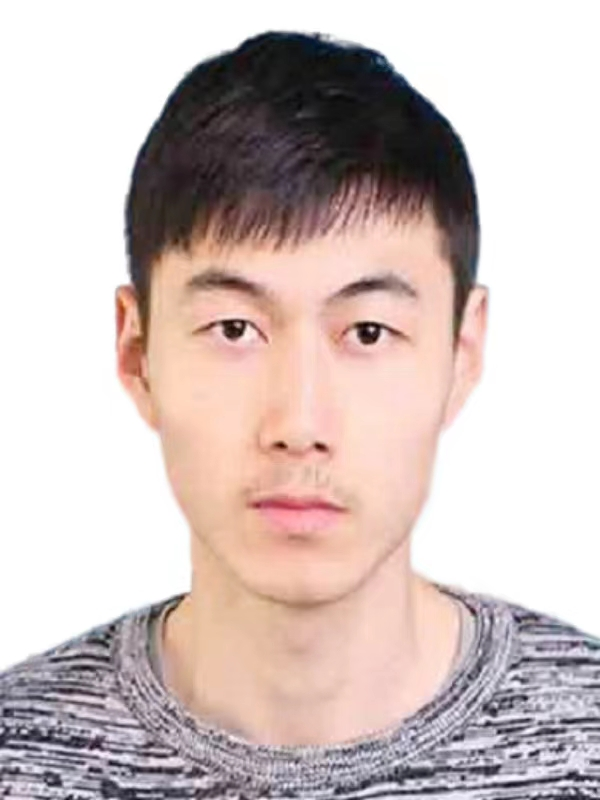
\includegraphics[width=1in,height=1.25in,clip,keepaspectratio]{figures/hyx.jpg}}]{Yuhang Huang}
received the bachelor’s degree from the University of Shanghai for Science and Technology, Shanghai, China, in 2019, and the master’s degree from Shanghai University, Shanghai, China, in 2022. He is currently pursuing the Ph.D. degree at the National University of Defense Technology, Changsha, China.

His research interests include computer vision, graphics, and generative models.
\end{IEEEbiography}


\vspace{11pt}
\begin{IEEEbiography}[{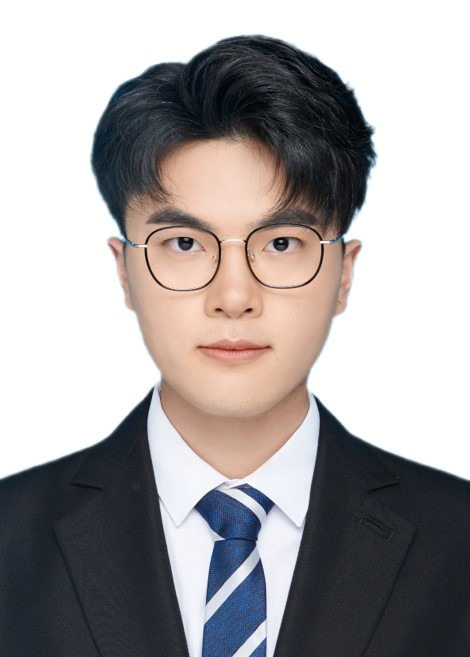
\includegraphics[width=1in,height=1.25in,clip,keepaspectratio]{figures/zsl.jpg}}]{Shilong Zou} received the bachelor's degree from the University of Dalian Maritime University, Dalian, 2023. He is currently pursuing the master's degree at the National University of Defense Technology, Changsha, China. 

His research interests include computer vision and generative models.
\end{IEEEbiography}
% \bf{If you will not include a photo:}\vspace{-33pt}
% \begin{IEEEbiographynophoto}{John Doe}
% Use $\backslash${\tt{begin\{IEEEbiographynophoto\}}} and the author name as the argument followed by the biography text.
% \end{IEEEbiographynophoto}
% \begin{IEEEbiography}[{\includegraphics[width=1in,height=1.25in,clip,keepaspectratio]{figures/qinzheng.jpg}}]{Zheng Qin} 
% received the PhD degree in computer science and technology from National University of Defense Technology (NUDT), China. He is currently an assistant professor with the Defense Innovation Institute, Academy of Military Sciences, China. His current research interests include 3D computer vision, 3D feature learning, shape modeling, and scene understanding.
% \end{IEEEbiography} 

% \vspace{11pt}
% \begin{IEEEbiography}[{\includegraphics[width=1in,height=1.25in,clip,keepaspectratio]{figures/xuesongxu.png}}]{Xuesong Xu} received his M.S and
% Ph.D. degree in Control Science and
% Engineering from Hunan University in
% 2004 and 2009 respectively. From 2012 to
% 2015, he works as a post-doctoral at
% National University of defense and
% technology. From 2016-2017, he also
% works as a visiting researcher in Volen
% National Center for Complex Systems,
% Brandeis University, USA. Currently, He is a professor of
% Hunan University of Technology and Business, working at
% Base of International Science and Technology Innovation and
% Cooperation on Big Data Technology and Management. His
% research interests are in the areas of complex system
% optimization, Blockchain and Machine learning. He has
% published more than 30 papers at various conferences and
% journals, including FGCS, Energy Reports, and Sensors. Prof.
% Xu is a member of the IEEE Computational Intelligence.
% \end{IEEEbiography}

% \vspace{11pt}
% \begin{IEEEbiography}[{\includegraphics[width=1in,height=1.25in,clip,keepaspectratio]{figures/zhuchengyang.png}}]{Chengyang Zhu} is an Associate Professor at the School of Computer, National University of Defense
% Technology. The current directions of interest include data-driven shape analysis and modeling, 3D vision and, robot perception \& navigation, etc.
% \end{IEEEbiography}

\vspace{11pt}
\begin{IEEEbiography}[{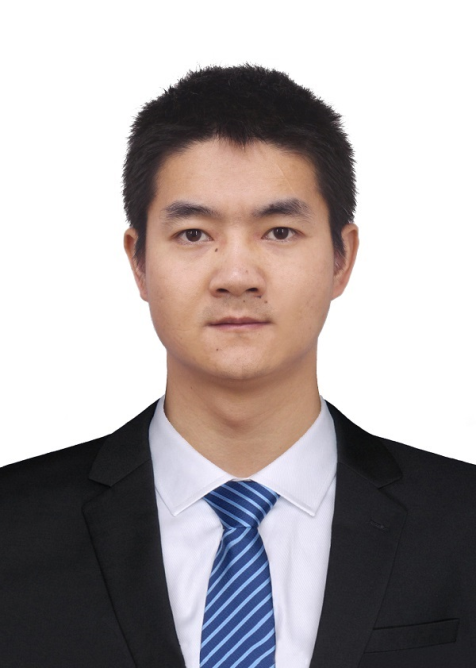
\includegraphics[width=1in,height=1.25in,clip,keepaspectratio]{figures/lxw.png}}]{Xinwang Liu}
received his PhD degree from National University of Defense Technology (NUDT), China. He is now Professor of School of Computer, NUDT. His current research interests include kernel learning and unsupervised feature learning. Dr. Liu has published 60+ peer-reviewed papers, including
those in highly regarded journals and conferences such as IEEE T-PAMI, IEEE T-KDE, IEEE T-IP, IEEE T-NNLS, IEEE T-MM, IEEE T-IFS, ICML, NeurIPS, ICCV, CVPR, AAAI, IJCAI, etc. He serves as the associated editor of Information Fusion Journal. More information can be found at \href{https://xinwangliu.github.io/}{https://xinwangliu.github.io/}.
\end{IEEEbiography}

% \begin{IEEEbiography}
% [{\includegraphics[width=1in,height=1.25in,clip,keepaspectratio]{figures/xiaohongchen.png}}]{Xiaohong Chen} 
% is an Academician of the Chinese Academy of Engineering and is a Distinguished Expert of Management Science and Engineering, Engineering Management, and Data Intelligence. Additionally, she is the Convener of the Management Science and Engineering Discipline Assessment Group under the Degree Committee of the State Council, the Director of the National Basic Science Center, and the Director of the Xiangjiang Laboratory, Changsha, China. Her leadership roles extend to the Innovation Group of the National Natural Science Foundation, the Cheung Kong Scholars Innovation Team under the Ministry of Education, and as a Leading Talent of Philosophy and Social Sciences in the Ten Thousand Talents Plan of the Organization Department of the Central Committee of the People’s Republic of China. She has published over 400 papers in prestigious academic journals, with more than 60 papers featured in the top 1\% of ESI highly cited papers, and holds an H-Index of 87. Her research focuses on decision theory and decision support systems, data intelligence, and the advancement of a smart society.
% \end{IEEEbiography}

\vspace{11pt}
\begin{IEEEbiography}[{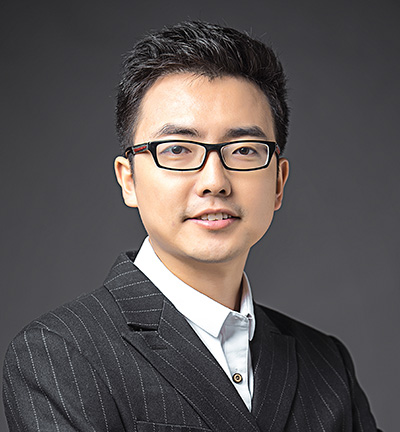
\includegraphics[width=1in,height=1.25in,clip,keepaspectratio]{figures/kevinxu.jpg}}]{Kai Xu} (Senior Member, IEEE) received the Ph.D. degree in computer science from the National University of Defense Technology (NUDT), Changsha,
China, in 2011. From 2008 to 2010, he worked as a Visiting Ph.D. degree with the GrUVi Laboratory, Simon Fraser University, Burnaby, BC, Canada. He is currently a Professor with the School of Computer Science, NUDT. He is also an Adjunct Professor with Simon Fraser University. His current research interests include data-driven shape analysis and modeling, and 3-D vision and robot perception and navigation.
\end{IEEEbiography}




\vfill

\end{document}



% \bibitem{ref1}
% {\it{Mathematics Into Type}}. American Mathematical Society. [Online]. Available: https://www.ams.org/arc/styleguide/mit-2.pdf

% \bibitem{ref2}
% T. W. Chaundy, P. R. Barrett and C. Batey, {\it{The Printing of Mathematics}}. London, U.K., Oxford Univ. Press, 1954.

% \bibitem{ref3}
% F. Mittelbach and M. Goossens, {\it{The \LaTeX Companion}}, 2nd ed. Boston, MA, USA: Pearson, 2004.

% \bibitem{ref4}
% G. Gr\"atzer, {\it{More Math Into LaTeX}}, New York, NY, USA: Springer, 2007.

% \bibitem{ref5}M. Letourneau and J. W. Sharp, {\it{AMS-StyleGuide-online.pdf,}} American Mathematical Society, Providence, RI, USA, [Online]. Available: http://www.ams.org/arc/styleguide/index.html

% \bibitem{ref6}
% H. Sira-Ramirez, ``On the sliding mode control of nonlinear systems,'' \textit{Syst. Control Lett.}, vol. 19, pp. 303--312, 1992.

% \bibitem{ref7}
% A. Levant, ``Exact differentiation of signals with unbounded higher derivatives,''  in \textit{Proc. 45th IEEE Conf. Decis.
% Control}, San Diego, CA, USA, 2006, pp. 5585--5590. DOI: 10.1109/CDC.2006.377165.

% \bibitem{ref8}
% M. Fliess, C. Join, and H. Sira-Ramirez, ``Non-linear estimation is easy,'' \textit{Int. J. Model., Ident. Control}, vol. 4, no. 1, pp. 12--27, 2008.

% \bibitem{ref9}
% R. Ortega, A. Astolfi, G. Bastin, and H. Rodriguez, ``Stabilization of food-chain systems using a port-controlled Hamiltonian description,'' in \textit{Proc. Amer. Control Conf.}, Chicago, IL, USA,
% 2000, pp. 2245--2249.

% \end{thebibliography}


\newpage

 
\vspace{11pt}

% \bf{If you include a photo:}\vspace{-33pt}
\begin{IEEEbiography}[{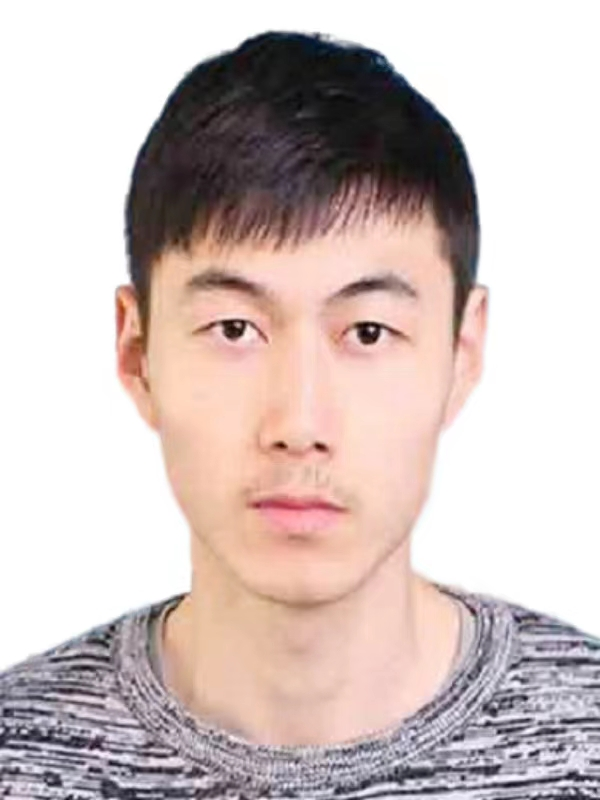
\includegraphics[width=1in,height=1.25in,clip,keepaspectratio]{figures/hyx.jpg}}]{Yuhang Huang}
received the bachelor’s degree from the University of Shanghai for Science and Technology, Shanghai, China, in 2019, and the master’s degree from Shanghai University, Shanghai, China, in 2022. He is currently pursuing the Ph.D. degree at the National University of Defense Technology, Changsha, China.

His research interests include computer vision, graphics, and generative models.
\end{IEEEbiography}


\vspace{11pt}
\begin{IEEEbiography}[{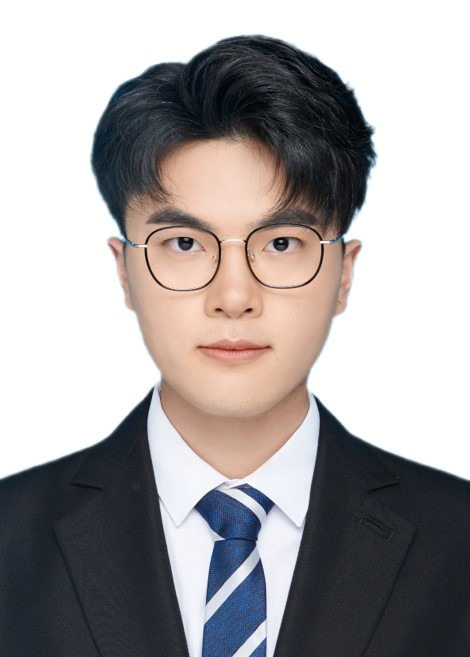
\includegraphics[width=1in,height=1.25in,clip,keepaspectratio]{figures/zsl.jpg}}]{Shilong Zou} received the bachelor's degree from the University of Dalian Maritime University, Dalian, 2023. He is currently pursuing the master's degree at the National University of Defense Technology, Changsha, China. 

His research interests include computer vision and generative models.
\end{IEEEbiography}
% \bf{If you will not include a photo:}\vspace{-33pt}
% \begin{IEEEbiographynophoto}{John Doe}
% Use $\backslash${\tt{begin\{IEEEbiographynophoto\}}} and the author name as the argument followed by the biography text.
% \end{IEEEbiographynophoto}
% \begin{IEEEbiography}[{\includegraphics[width=1in,height=1.25in,clip,keepaspectratio]{figures/qinzheng.jpg}}]{Zheng Qin} 
% received the PhD degree in computer science and technology from National University of Defense Technology (NUDT), China. He is currently an assistant professor with the Defense Innovation Institute, Academy of Military Sciences, China. His current research interests include 3D computer vision, 3D feature learning, shape modeling, and scene understanding.
% \end{IEEEbiography} 

% \vspace{11pt}
% \begin{IEEEbiography}[{\includegraphics[width=1in,height=1.25in,clip,keepaspectratio]{figures/xuesongxu.png}}]{Xuesong Xu} received his M.S and
% Ph.D. degree in Control Science and
% Engineering from Hunan University in
% 2004 and 2009 respectively. From 2012 to
% 2015, he works as a post-doctoral at
% National University of defense and
% technology. From 2016-2017, he also
% works as a visiting researcher in Volen
% National Center for Complex Systems,
% Brandeis University, USA. Currently, He is a professor of
% Hunan University of Technology and Business, working at
% Base of International Science and Technology Innovation and
% Cooperation on Big Data Technology and Management. His
% research interests are in the areas of complex system
% optimization, Blockchain and Machine learning. He has
% published more than 30 papers at various conferences and
% journals, including FGCS, Energy Reports, and Sensors. Prof.
% Xu is a member of the IEEE Computational Intelligence.
% \end{IEEEbiography}

% \vspace{11pt}
% \begin{IEEEbiography}[{\includegraphics[width=1in,height=1.25in,clip,keepaspectratio]{figures/zhuchengyang.png}}]{Chengyang Zhu} is an Associate Professor at the School of Computer, National University of Defense
% Technology. The current directions of interest include data-driven shape analysis and modeling, 3D vision and, robot perception \& navigation, etc.
% \end{IEEEbiography}

\vspace{11pt}
\begin{IEEEbiography}[{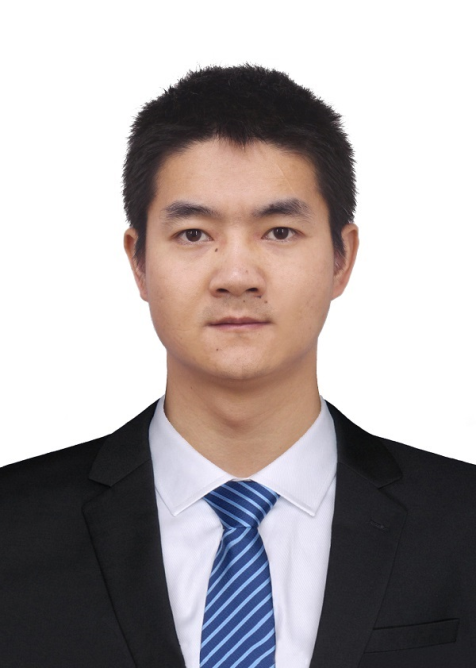
\includegraphics[width=1in,height=1.25in,clip,keepaspectratio]{figures/lxw.png}}]{Xinwang Liu}
received his PhD degree from National University of Defense Technology (NUDT), China. He is now Professor of School of Computer, NUDT. His current research interests include kernel learning and unsupervised feature learning. Dr. Liu has published 60+ peer-reviewed papers, including
those in highly regarded journals and conferences such as IEEE T-PAMI, IEEE T-KDE, IEEE T-IP, IEEE T-NNLS, IEEE T-MM, IEEE T-IFS, ICML, NeurIPS, ICCV, CVPR, AAAI, IJCAI, etc. He serves as the associated editor of Information Fusion Journal. More information can be found at \href{https://xinwangliu.github.io/}{https://xinwangliu.github.io/}.
\end{IEEEbiography}

% \begin{IEEEbiography}
% [{\includegraphics[width=1in,height=1.25in,clip,keepaspectratio]{figures/xiaohongchen.png}}]{Xiaohong Chen} 
% is an Academician of the Chinese Academy of Engineering and is a Distinguished Expert of Management Science and Engineering, Engineering Management, and Data Intelligence. Additionally, she is the Convener of the Management Science and Engineering Discipline Assessment Group under the Degree Committee of the State Council, the Director of the National Basic Science Center, and the Director of the Xiangjiang Laboratory, Changsha, China. Her leadership roles extend to the Innovation Group of the National Natural Science Foundation, the Cheung Kong Scholars Innovation Team under the Ministry of Education, and as a Leading Talent of Philosophy and Social Sciences in the Ten Thousand Talents Plan of the Organization Department of the Central Committee of the People’s Republic of China. She has published over 400 papers in prestigious academic journals, with more than 60 papers featured in the top 1\% of ESI highly cited papers, and holds an H-Index of 87. Her research focuses on decision theory and decision support systems, data intelligence, and the advancement of a smart society.
% \end{IEEEbiography}

\vspace{11pt}
\begin{IEEEbiography}[{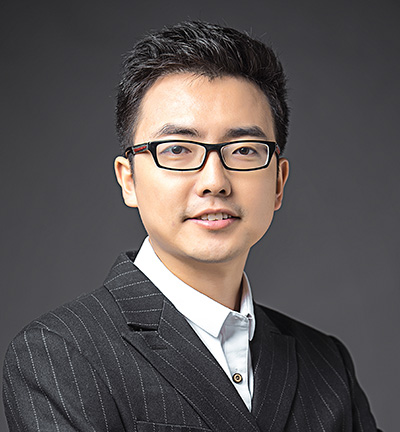
\includegraphics[width=1in,height=1.25in,clip,keepaspectratio]{figures/kevinxu.jpg}}]{Kai Xu} (Senior Member, IEEE) received the Ph.D. degree in computer science from the National University of Defense Technology (NUDT), Changsha,
China, in 2011. From 2008 to 2010, he worked as a Visiting Ph.D. degree with the GrUVi Laboratory, Simon Fraser University, Burnaby, BC, Canada. He is currently a Professor with the School of Computer Science, NUDT. He is also an Adjunct Professor with Simon Fraser University. His current research interests include data-driven shape analysis and modeling, and 3-D vision and robot perception and navigation.
\end{IEEEbiography}




\vfill

\end{document}


